\chapter{Tiling the Sky}
\label{chap:tiling}
\chaptoc{}

% ########################################

\newpage
\section{Introduction}
\label{sec:tiling_intro}
\begin{colsection}

In this chapter I describe the software used by GOTO to create an all-sky survey grid, which gravitational-wave events are then mapped onto.
%
\begin{itemize}
    \item In \nref{sec:gototile} I describe the GOTO-tile Python package, and the algorithms is uses to define the GOTO all-sky survey grid.
    \item In \nref{sec:skymaps} I describe how transient alert localisations are defined using skymaps and how they are mapped onto the GOTO-tile grid.
    \item In \nref{sec:custom_skymaps} I give some examples of how other skymaps can be used to direct GOTO observations.
\end{itemize}
%
All work described in this chapter is my own unless otherwise indicated, and has not been published elsewhere. The original GOTO-tile package was written by Darren White at Sheffield and Evert Rol at Monash, before I took over development and made substantial changes described in this chapter.

\end{colsection}

% ########################################

\newpage
\section{Defining the sky grid}
\label{sec:gototile}
\begin{colsection}

% ~~~~~~~~~~~~~~~~~~~~

\begin{colsection}

GOTO-tile is a Python package (\pkg{gototile}\footnote{\url{https://github.com/GOTO-OBS/goto-tile}}) created for the GOTO project to contain all of the functions related to tiling the sky and processing skymaps. It was originally developed by Darren White as a way to process gravitational-wave skymaps for GOTO, and then maintained by Evert Rol who rearranged it into a package usable for some other telescopes including SuperWASP on La Palma and a proposed southern GOTO node. My contributions to the package have been extensive: reworking the foundations to improve how the sky grid is defined and skymaps are applied, as well as adding additional code to create new skymaps (described in \aref{sec:grb_skymaps}).

\end{colsection}

% ~~~~~~~~~~~~~~~~~~~~

\subsection{Creating sky grids}
\label{sec:grids}
\begin{colsection}

The core of GOTO-tile as it now exists is the \code{SkyGrid} Python class, which is used to define a sky grid: a collection of regularly-spaced points on the celestial sphere. These points are used as the centre of rectangular `tiles' aligned to the equatorial right ascension/declination coordinate system, which create a framework for survey observations to be mapped on to.

The most important parameter required when defining a sky grid is the field of view of the telescope, which is taken as the size of the tiles that make up the grid. The field of view is defined within GOTO-tile by giving a width and height value in degrees, meaning the tiles can only be square or rectangular. This is typically fine for the GOTO array, which has a total field of view comprising of overlapping rectangles from each unit telescope (see \aref{fig:fov}). There was a period when having three unit telescopes in an `L'-shape was considered, but this was abandoned due mainly to the complexity of tiling the grid based on abstract shapes. For the prototype 4-UT GOTO system currently on La Palma a rectangular \SI{3.7}{\degree} $\times$ \SI{4.9}{\degree} tile was defined during commissioning, see \aref{fig:4ut_footprint}.

The second parameter required to define a sky grid is the desired overlap between the tiles. This is given as a value between zero and one in both the right ascension and declination axes, with zero meaning no overlap and one meaning all the tiles are completely overlapping (in practice the overlap is restricted to no more than $0.9$). The overlap is used to define the spacing between the tile centres, depending on the algorithm used. The current 4-UT grid uses an overlap of 0.1 (10\%) in both axes.

As GOTO-tile has been developed the algorithm used to define the grid has changed (see \aref{sec:algorithms}), but the basic method remained the same:

\begin{enumerate}
    \item On the celestial sphere (\aref{fig:sphere}) equally spaced lines of constant declination are defined, separated by the value $\Delta\delta$ (\aref{fig:deltadelta}). These ``declination strips'' are the basis for the grid points, which the tiles are centred on.
    \item Each declination strip is then filled with equally spaced points separated by the value $\Delta\alpha$ (\aref{fig:deltaalpha}). This value is constant within each strip but is (in most algorithms) a function of declination $\Delta\alpha(\delta)$, meaning that as one moves away from the equator towards the poles each strip will contain a fewer number of points.
    \item These points are then defined as the centres of the tiles, the size of which is given by the field of view (\aref{fig:tiledsphere}).
\end{enumerate}

Once the grid has been created it is encapsulated within the GOTO-tile \code{SkyGrid} class. Each tile is defined by a coordinate at its centre, and each is also given a unique name of the form \code{T0001}. The grid itself is also given a name formed using the input field of view and overlap parameters, so the current  grid (with a field of view of \SI{3.7}{\degree}$\times$\SI{4.9}{\degree} and overlap factor of 0.1 in both axes) is given the name \code{allsky-3.7x4.9--0.1--0.1}. In this way a given tile in a given grid can be recreated just from the grid and tile name, which is used when storing the details in the \code{grids} and \code{grid\_tiles} tables in observation database (see \aref{sec:obsdb}). % chktex 29

\newpage

% https://texfaq.org/FAQ-vertposfp
\makeatletter
\setlength{\@fptop}{0pt}
\makeatother

\begin{figure}[t]
    \begin{center}
        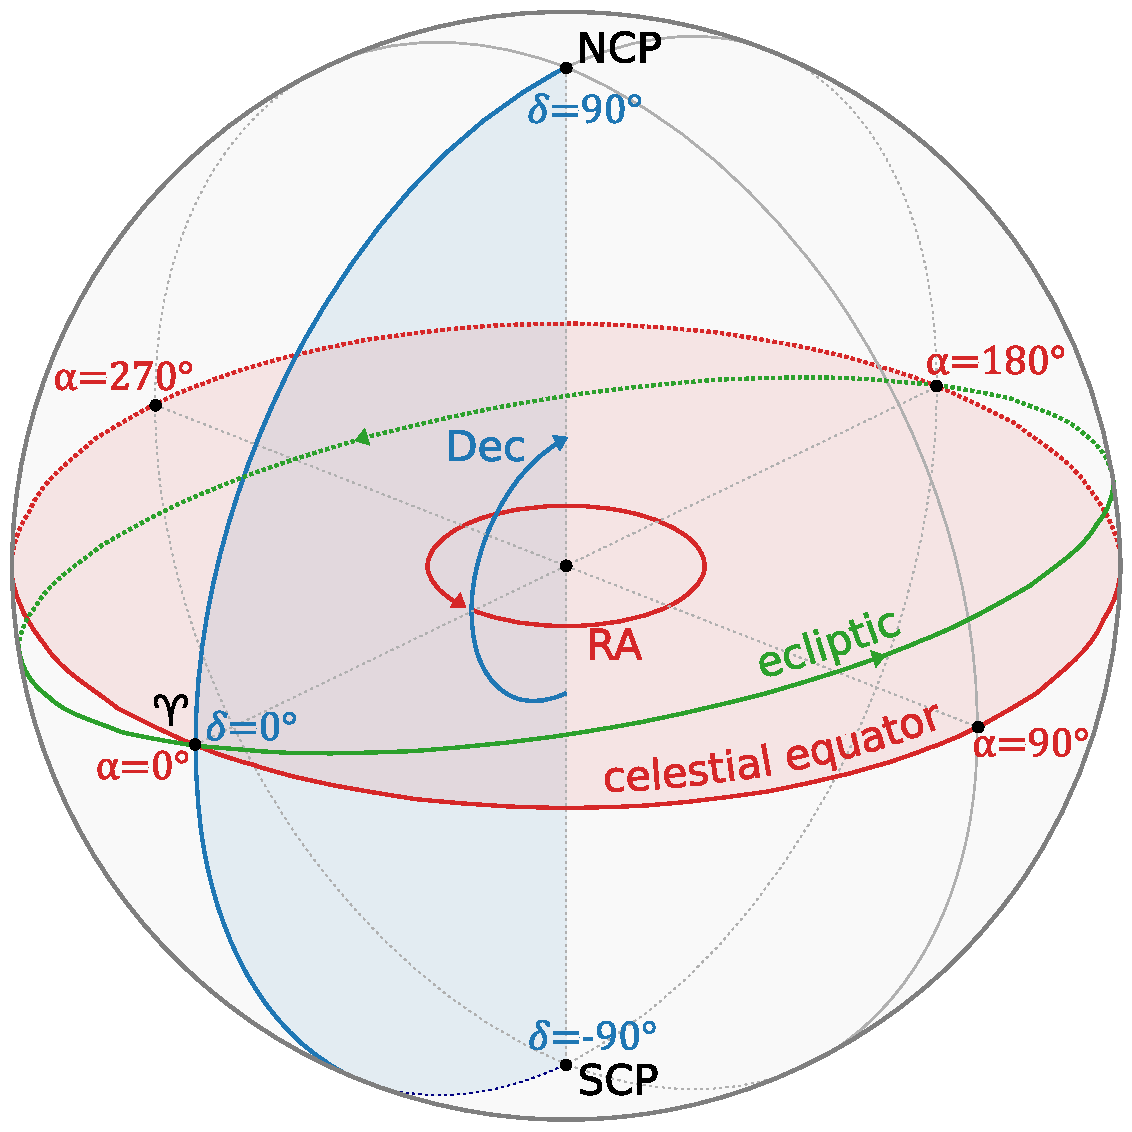
\includegraphics[width=\linewidth]{images/globe1.pdf}
    \end{center}
    \caption[The celestial sphere]{
        The celestial sphere. The northern and southern celestial poles are marked as \textbf{NCP} \glsadd{ncp} and \textbf{SCP} \glsadd{scp} respectively, and the celestial equator is marked in \textcolorbf{Red}{red}. The ecliptic (the path of the Sun) is marked in \textcolorbf{Green}{green}, the point where the ecliptic rises above the celestial equator (the vernal equinox) is marked with the symbol \Aries{}, and the meridian that intercepts the poles and the vernal equinox is marked in \textcolorbf{NavyBlue}{blue}.\\
        Traditionally the equatorial coordinate system defined as shown: declination (\textcolorbf{NavyBlue}{Dec}, $\delta$) is the angle from the equator (between \SI{-90}{\degree} at the SCP to \SI{90}{\degree} at the NCP) and right ascension (\textcolorbf{Red}{RA}, $\alpha$) \glsadd{ra} is the angle east of the vernal equinox (between \SI{0}{\degree} and \SI{360}{\degree}). \\
        The modern \glsfirst{icrs} defines coordinates based on radio sources which approximately match the ones described here \citep{ICRF}.
    }\label{fig:sphere}
\end{figure}

\clearpage

\begin{figure}[t]
    \begin{center}
        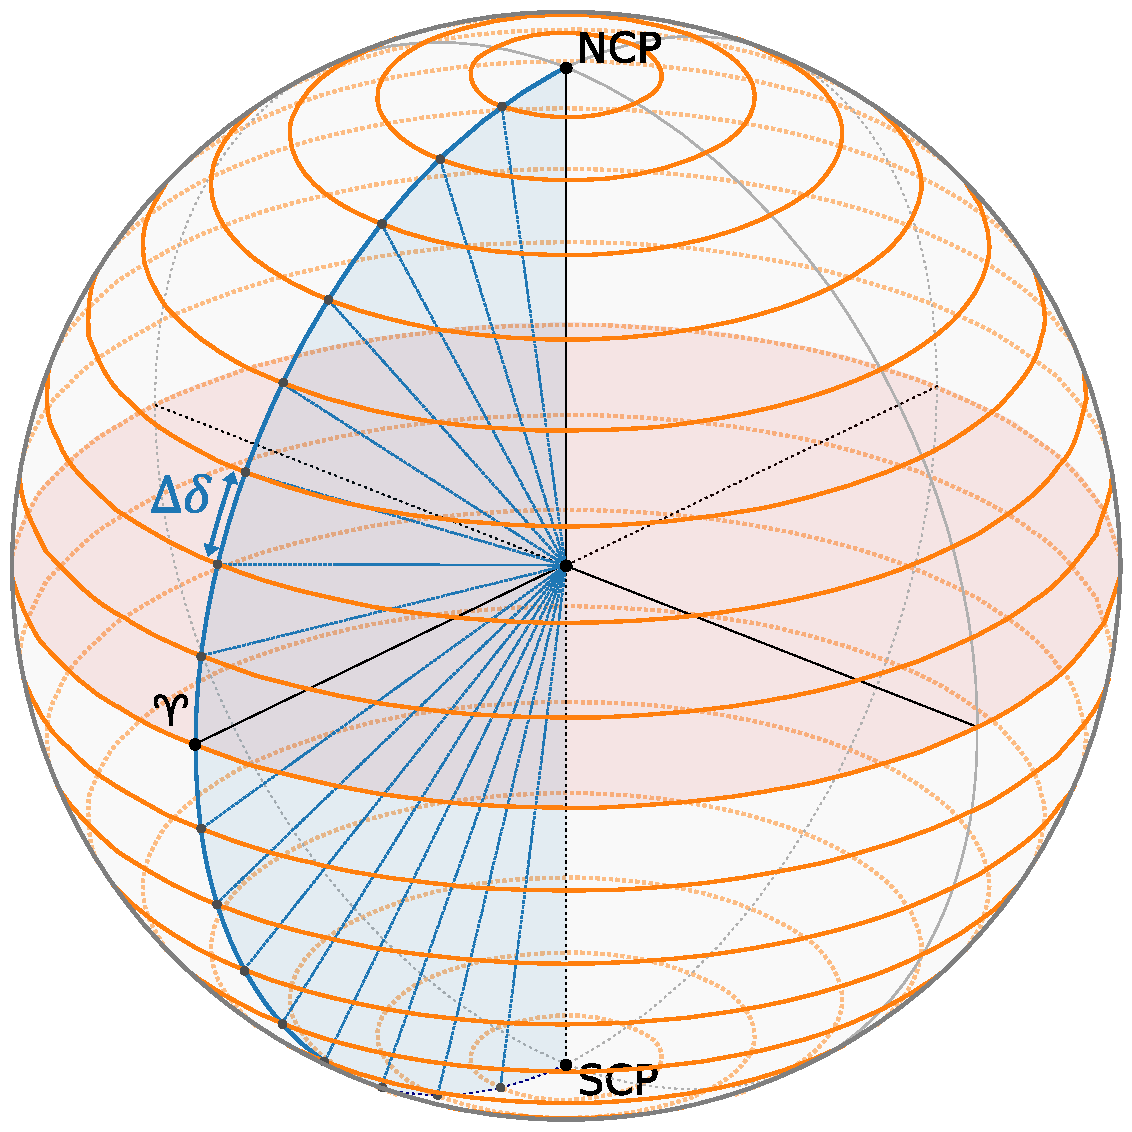
\includegraphics[width=\linewidth]{images/globe2.pdf}
    \end{center}
    \caption[Defining declination strips]{
        Defining the declination strips (shown in \textcolorbf{Orange}{orange}). The full declination range (\SI{-90}{\degree} to \SI{90}{\degree}) is divided equally by a constant spacing value $\Delta\delta$ (in \textcolorbf{NavyBlue}{blue}). \\
        In this example $\Delta\delta =$ \SI{10}{\degree}, and so the centre of each strip is set at $\delta=$ \SI{0}{\degree}, $\pm$\SI{10}{\degree}, $\pm$\SI{20}{\degree} etc. This gives 19 strips, 9 in each hemisphere and one on the equator. There is always a strip centred on $\delta=0$, and using the ``minverlap'' algorithm (see \aref{sec:algorithms}) there is always a `strip' of tiles at the poles which will include a single point.
    }\label{fig:deltadelta}
\end{figure}

\clearpage

\begin{figure}[t]
    \begin{center}
        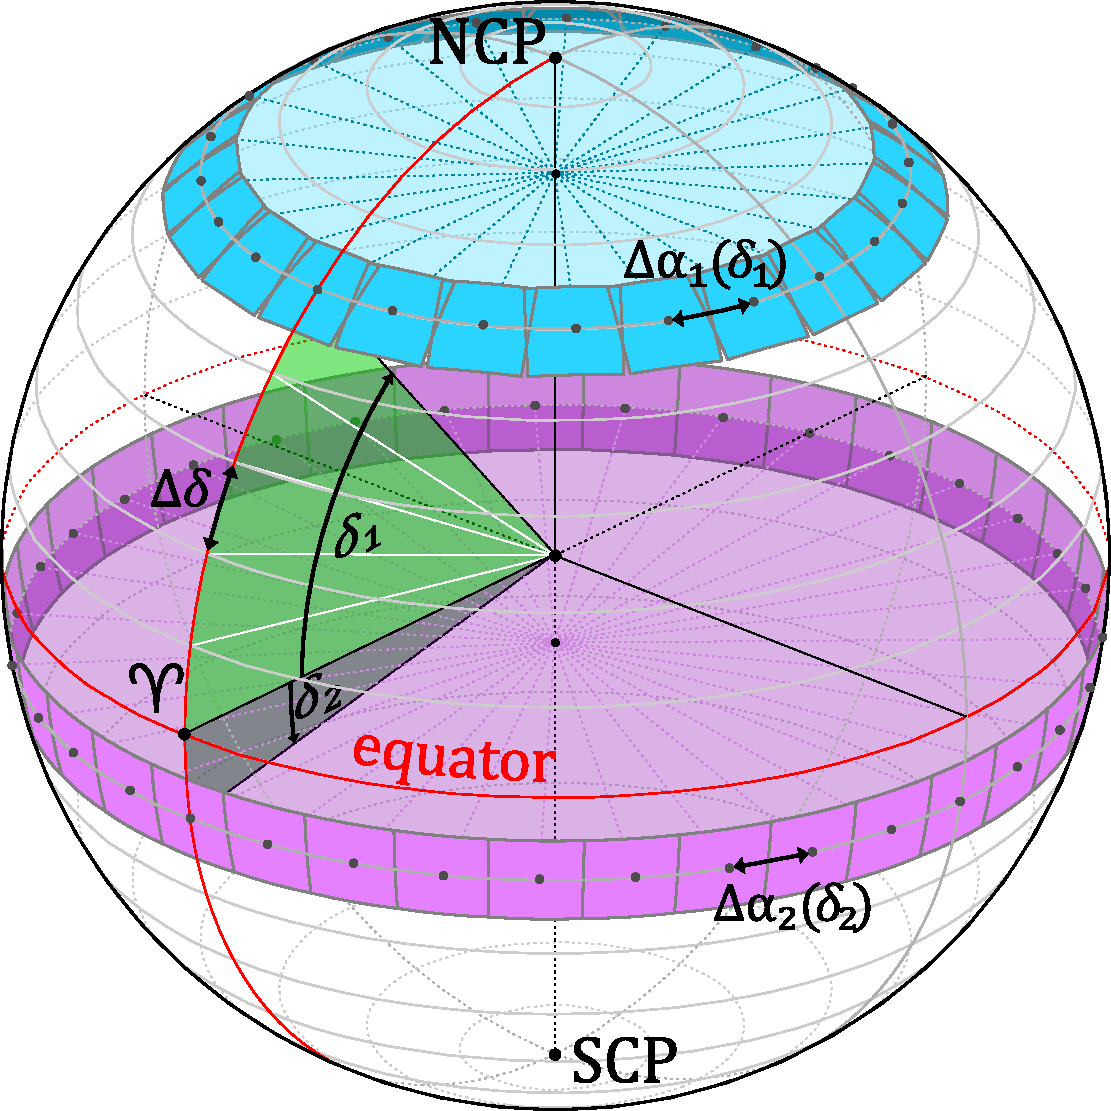
\includegraphics[width=\linewidth]{images/globe3.pdf}
    \end{center}
    \caption[Defining grid points]{
        Defining the grid points, based on the declination strips from \aref{fig:deltadelta}. Using the ``minverlap'' algorithm (see \aref{sec:algorithms}) points are uniformly distributed on each declination strip with a spacing $\Delta\alpha(\delta)$. Unlike $\Delta\delta$, which is fixed across the sphere, $\Delta\alpha$ varies as a function of declination, meaning strips closer to the poles will contain fewer points (and therefore fewer tiles). \\
        Two examples of defining grid points are shown, one at declination $\delta_1=+$\SI{50}{\degree} (in \textcolorbf{Purple}{purple}) in the northern hemisphere and another at $\delta_2=-$\SI{10}{\degree} (in \textcolorbf{BlueGreen}{cyan}) in the southern hemisphere. The survey tiles are then centred on the grid points, as shown for these two strips.
    }\label{fig:deltaalpha}
\end{figure}

\clearpage

\begin{figure}[t]
    \begin{center}
        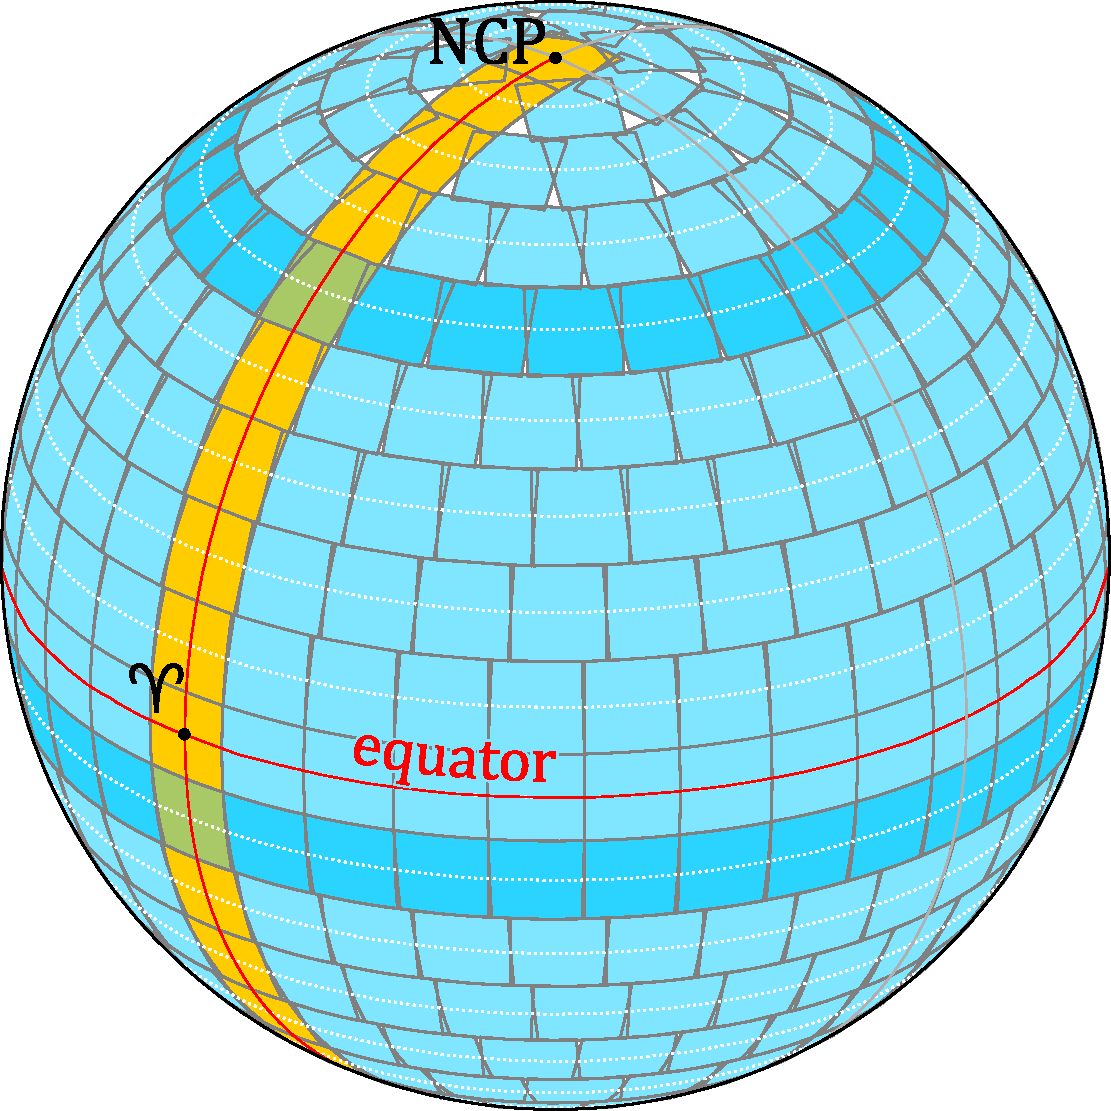
\includegraphics[width=\linewidth]{images/globe4.pdf}
    \end{center}
    \caption[A fully tiled celestial sphere]{
        A fully tiled celestial sphere. The same two strips of tiles are coloured in \textcolorbf{Purple}{purple} and \textcolorbf{BlueGreen}{cyan} as in \aref{fig:deltaalpha}. As each strip starts with a tile at RA$=0$ there is a fully aligned column of tiles along the meridian through the vernal equinox, coloured in \textcolorbf{YellowOrange}{yellow}, and there is always a tile centred on the vernal equinox and each pole. \\
        This grid was defined using the ``minverlap'' algorithm (see \aref{sec:algorithms}), with each tile having a field of view of \SI{10}{\degree} $\times$ \SI{10}{\degree} and a overlap of zero for clarity. Note zero overlap can lead to gaps between tiles towards the poles, shown by the \textcolorbf{Red}{red} patches. In this case the complete grid contains 424 tiles.
    }\label{fig:tiledsphere}
\end{figure}

\clearpage

% https://tex.stackexchange.com/questions/28556/how-to-place-a-float-at-the-top-of-a-floats-only-page
\makeatletter
\setlength{\@fptop}{0\p@ \@plus 1fil} % chktex 1
\makeatother

\end{colsection}

% ~~~~~~~~~~~~~~~~~~~~

\subsection{Different gridding algorithms}
\label{sec:algorithms}
\begin{colsection}

There have been three different algorithms used by GOTO-tile to define the grid.

% ---------
\subsubsection{The product algorithm}

The first has since retroactively been called the ``\textbf{product}'' algorithm, and was used when Darren White first wrote GOTO-tile. It first defines the declination step size as
%
\begin{equation}
    \Delta\delta = f_\text{dec}(1-v_\text{dec}),
    \label{eq:product_deltadelta}
\end{equation}
%
where $f_\text{dec}$ and $v_\text{dec}$ are respectively the field of view in degrees and the fractional overlap parameters in the declination direction. The declination strips are then defined by taking steps of this size from the equator towards the poles, stopping when $|\delta| > 90$. An equivalent formula is used to calculate the steps in right ascension

\begin{equation}
    \Delta\alpha = f_\text{RA}(1-v_\text{RA}).
    \label{eq:product_deltaalpha}
\end{equation}

The clear downside of this method is that $\Delta\alpha$ does not vary with declination. In effect this algorithm attempts to define the grid as if it was on a flat plane, where the tiles could be arranged in orthogonal rows and columns. In practice when applied to a sphere this leads to a vast number of redundant tiles at the poles, as shown in \aref{fig:product}.

% ---------
\subsubsection{The cosine algorithm}

Due to the obvious problems with the product algorithm, a replacement was written by Evert Rol, which I have since called the ``\textbf{cosine}'' algorithm. It is a more refined version of the product algorithm, and the declination strips are calculated in the same manner using \aref{eq:product_deltadelta}. However \aref{eq:product_deltaalpha} is modified to depend on declination:
%
\begin{equation}
    \Delta\alpha(\delta) = \frac{f_\text{RA}(1-v_\text{RA})}{\cos \delta}.
    \label{eq:cosine_deltaalpha}
\end{equation}

This produces a more sensible grid with fewer redundant tiles at the poles, as shown in \aref{fig:cosine}. However, there remained an issue of asymmetry: the strips are arranged increasing and decreasing from $\delta=0$ and the tiles are then arranged within the strips starting from $\alpha=0$. This leads to varying levels of overlap when the tiles within the strips meet as $\alpha$ approaches \SI{360}{\degree}, as visible in \aref{fig:cosine}. Although more subtle, there are similar issues at the north and south celestial poles. It is also common for there to be small gaps between the tiles at high and low declinations.

% ---------
\subsubsection{The minverlap algorithm}

Due to these problems I created a new method to create the grid, called the ``\textbf{minverlap}'' (\emph{min}imum o\emph{verlap}) algorithm. A grid created with this algorithm is shown in \aref{fig:minverlap}. The intention of the new algorithm was to solve the issues with the product and cosine algorithms by dynamically adjusting the spacing between tiles. The previous two algorithms both treated the user-specified overlap parameter as fixed, and if the resulting spacings did not give an integer number of tiles within the ranges available then they produced uneven gaps at the edges. This is shown more clearly in \aref{fig:cosine_spacing}, where a particular spacing results in gaps at the celestial poles and variable overlaps across the RA$=0$ meridian.

The minverlap algorithm solves these problems by treating the overlap parameter not as fixed but as the \textit{minimum} required overlap between tiles. For example, if a grid is requested with an overlap of $0.2$ (20\%) but the field of view of the tiles does not neatly divide by \SI{90}{\degree} then the overlap can be increased until an integer number of tiles fit, as shown in \aref{fig:minverlap_spacing}.

\newpage

\begin{figure}[p]
    \begin{minipage}[c]{0.46\textwidth}
        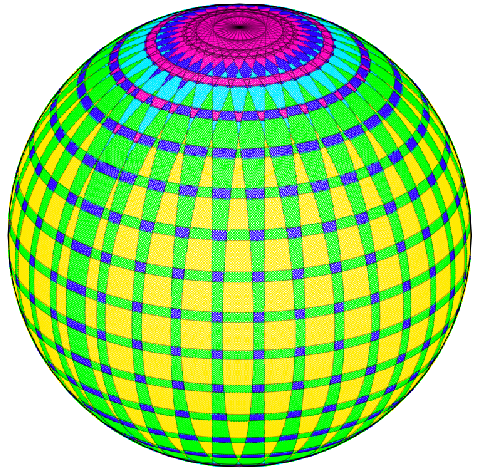
\includegraphics[width=\linewidth]{images/algo_product.pdf}
    \end{minipage}
    \hfill
    \begin{minipage}[c]{0.50\textwidth}
        \caption[The product gridding algorithm]{
            A sky grid of tiles defined using the ``product'' gridding algorithm. The inputs were a field of view of \SI{13}{\degree} $\times$ \SI{13}{\degree} and an overlap factor of $0.2$ in both axes. The colours show overlapping coverage: \textcolorbf{YellowOrange}{yellow} areas are within only one tile, \textcolorbf{ForestGreen}{green} two, \textcolorbf{blue}{blue} three, \textcolorbf{cyan}{cyan} four and \textcolorbf{RubineRed}{pink} five or more. This grid contains 595 tiles. Note the constant spacing of tiles in RA and the huge number of redundant tiles at the pole.
        }\label{fig:product}
    \end{minipage}
\end{figure}

\begin{figure}[p]
    \begin{minipage}[c]{0.50\textwidth}
        \caption[The cosine gridding algorithm]{
            A sky grid of tiles defined using the ``product'' gridding algorithm. The input parameters and colours are the same as in \aref{fig:product}. This grid contains 393 tiles. Note the asymmetric ``seam'' along the $\alpha=0$ meridian, and the \textcolorbf{red}{red} areas near the pole that are not within the area of any tiles.
        }\label{fig:cosine}
    \end{minipage}
    \hfill
    \begin{minipage}[c]{0.46\textwidth}
        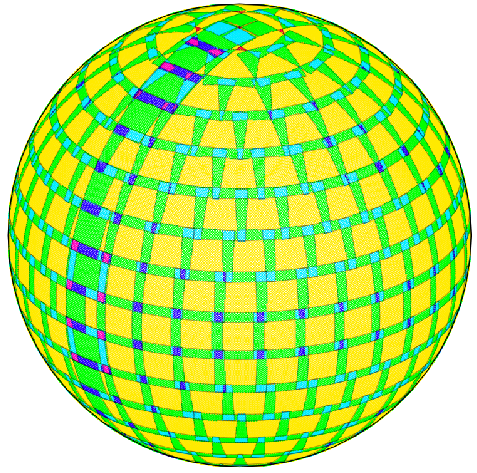
\includegraphics[width=\linewidth]{images/algo_cosine.pdf}
    \end{minipage}
\end{figure}

\begin{figure}[p]
    \begin{minipage}[c]{0.46\textwidth}
        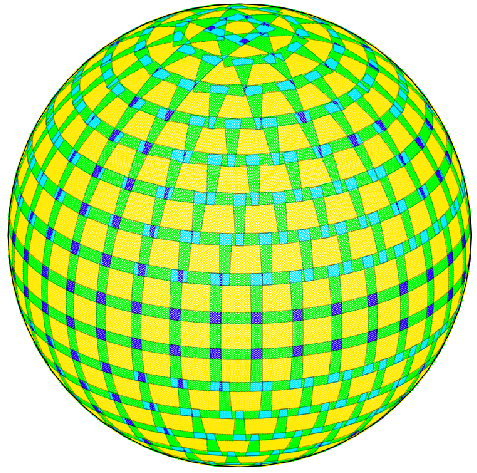
\includegraphics[width=\linewidth]{images/algo_minverlap.pdf}
    \end{minipage}
    \hfill
    \begin{minipage}[c]{0.50\textwidth}
        \caption[The minverlap gridding algorithm]{
            A sky grid of tiles defined using the ``minverlap'' gridding algorithm. The input parameters and colours are the same as in \aref{fig:product}. This grid contains 407 tiles. Note the even spacing of tiles even over the $\alpha=0$ meridian, and the better coverage at the pole.
        }\label{fig:minverlap}
    \end{minipage}
\end{figure}

\newpage

\begin{figure}[p]
    \begin{center}
        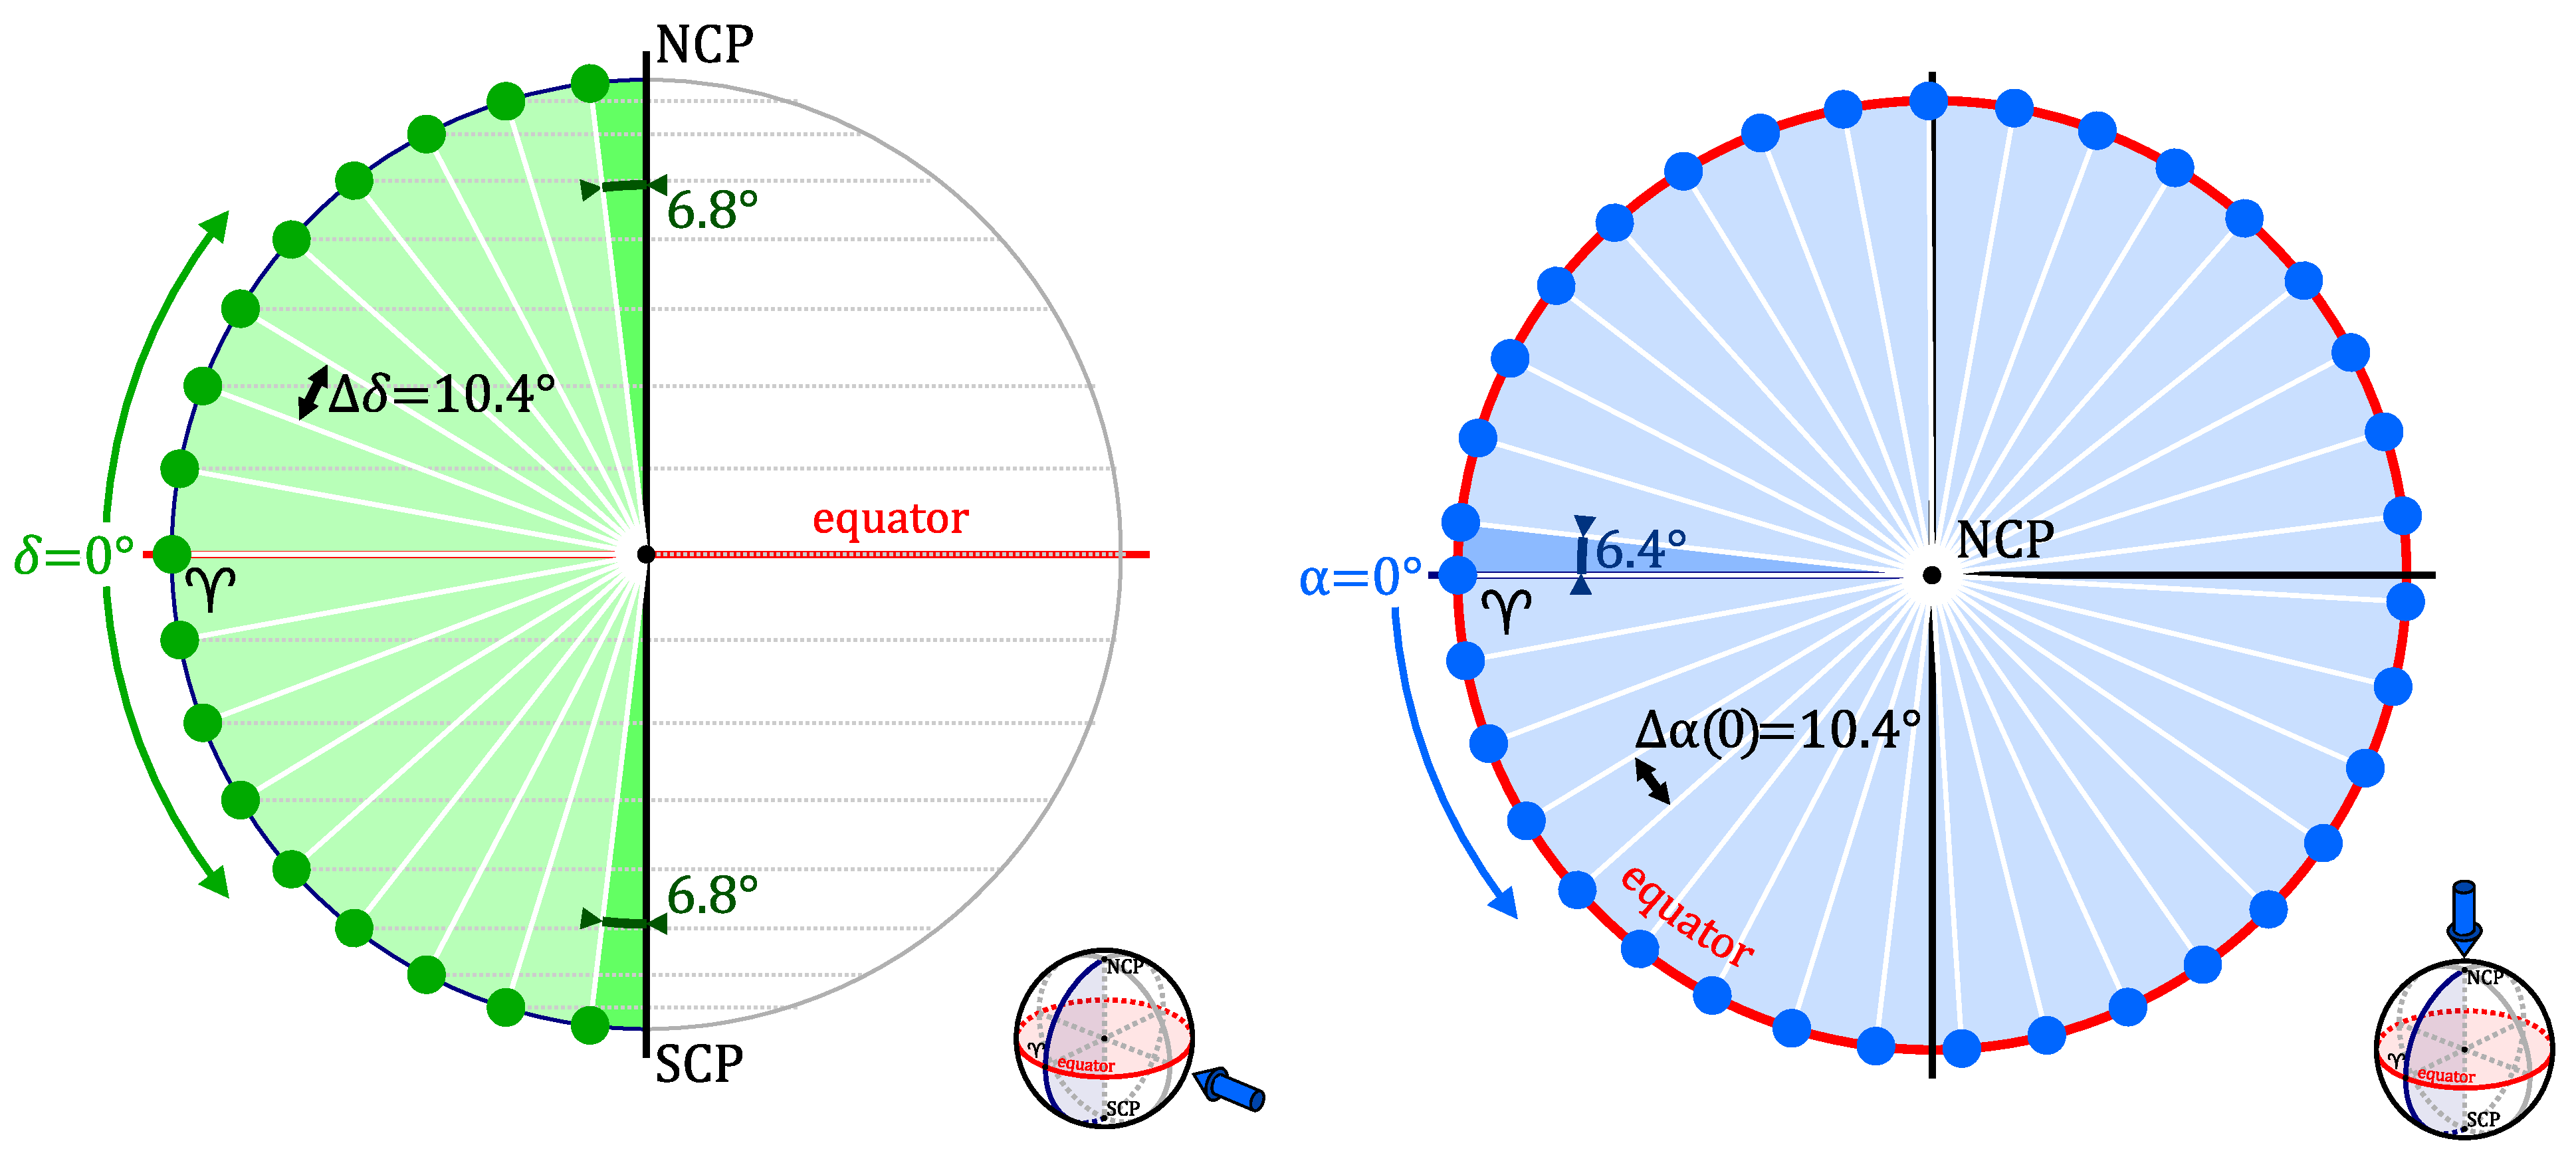
\includegraphics[width=\linewidth]{images/spacing_cosine.pdf}
    \end{center}
    \caption[Grid spacing with the cosine algorithm]{
        Grid spacing with the cosine algorithm. Using a \SI{13}{\degree}$\times$\SI{13}{\degree} field of view and an overlap of $0.2$ \aref{eq:product_deltadelta} gives $\Delta\delta = $ \SI{10.4}{\degree}. 17 declination strips are defined moving away from $\delta=0$, as shown in the equatorial view on the left. The final strips are \SI{6.8}{\degree} from the poles, as this is more than half of the field of view (\SI{6.5}{\degree}) the poles themselves will not by within the area of any tile. \aref{eq:cosine_deltaalpha} gives $\Delta\alpha = $ \SI{10.4}{\degree} on the equator ($\delta=0$). This results in 35 points arranged as shown in the polar view on the right, and a reduced spacing of \SI{6.4}{\degree} to the west of the $\alpha=0$ meridian. This remainder will be different for each strip, as shown in \aref{fig:cosine}.
    }\label{fig:cosine_spacing}
\end{figure}

\begin{figure}[p]
    \begin{center}
        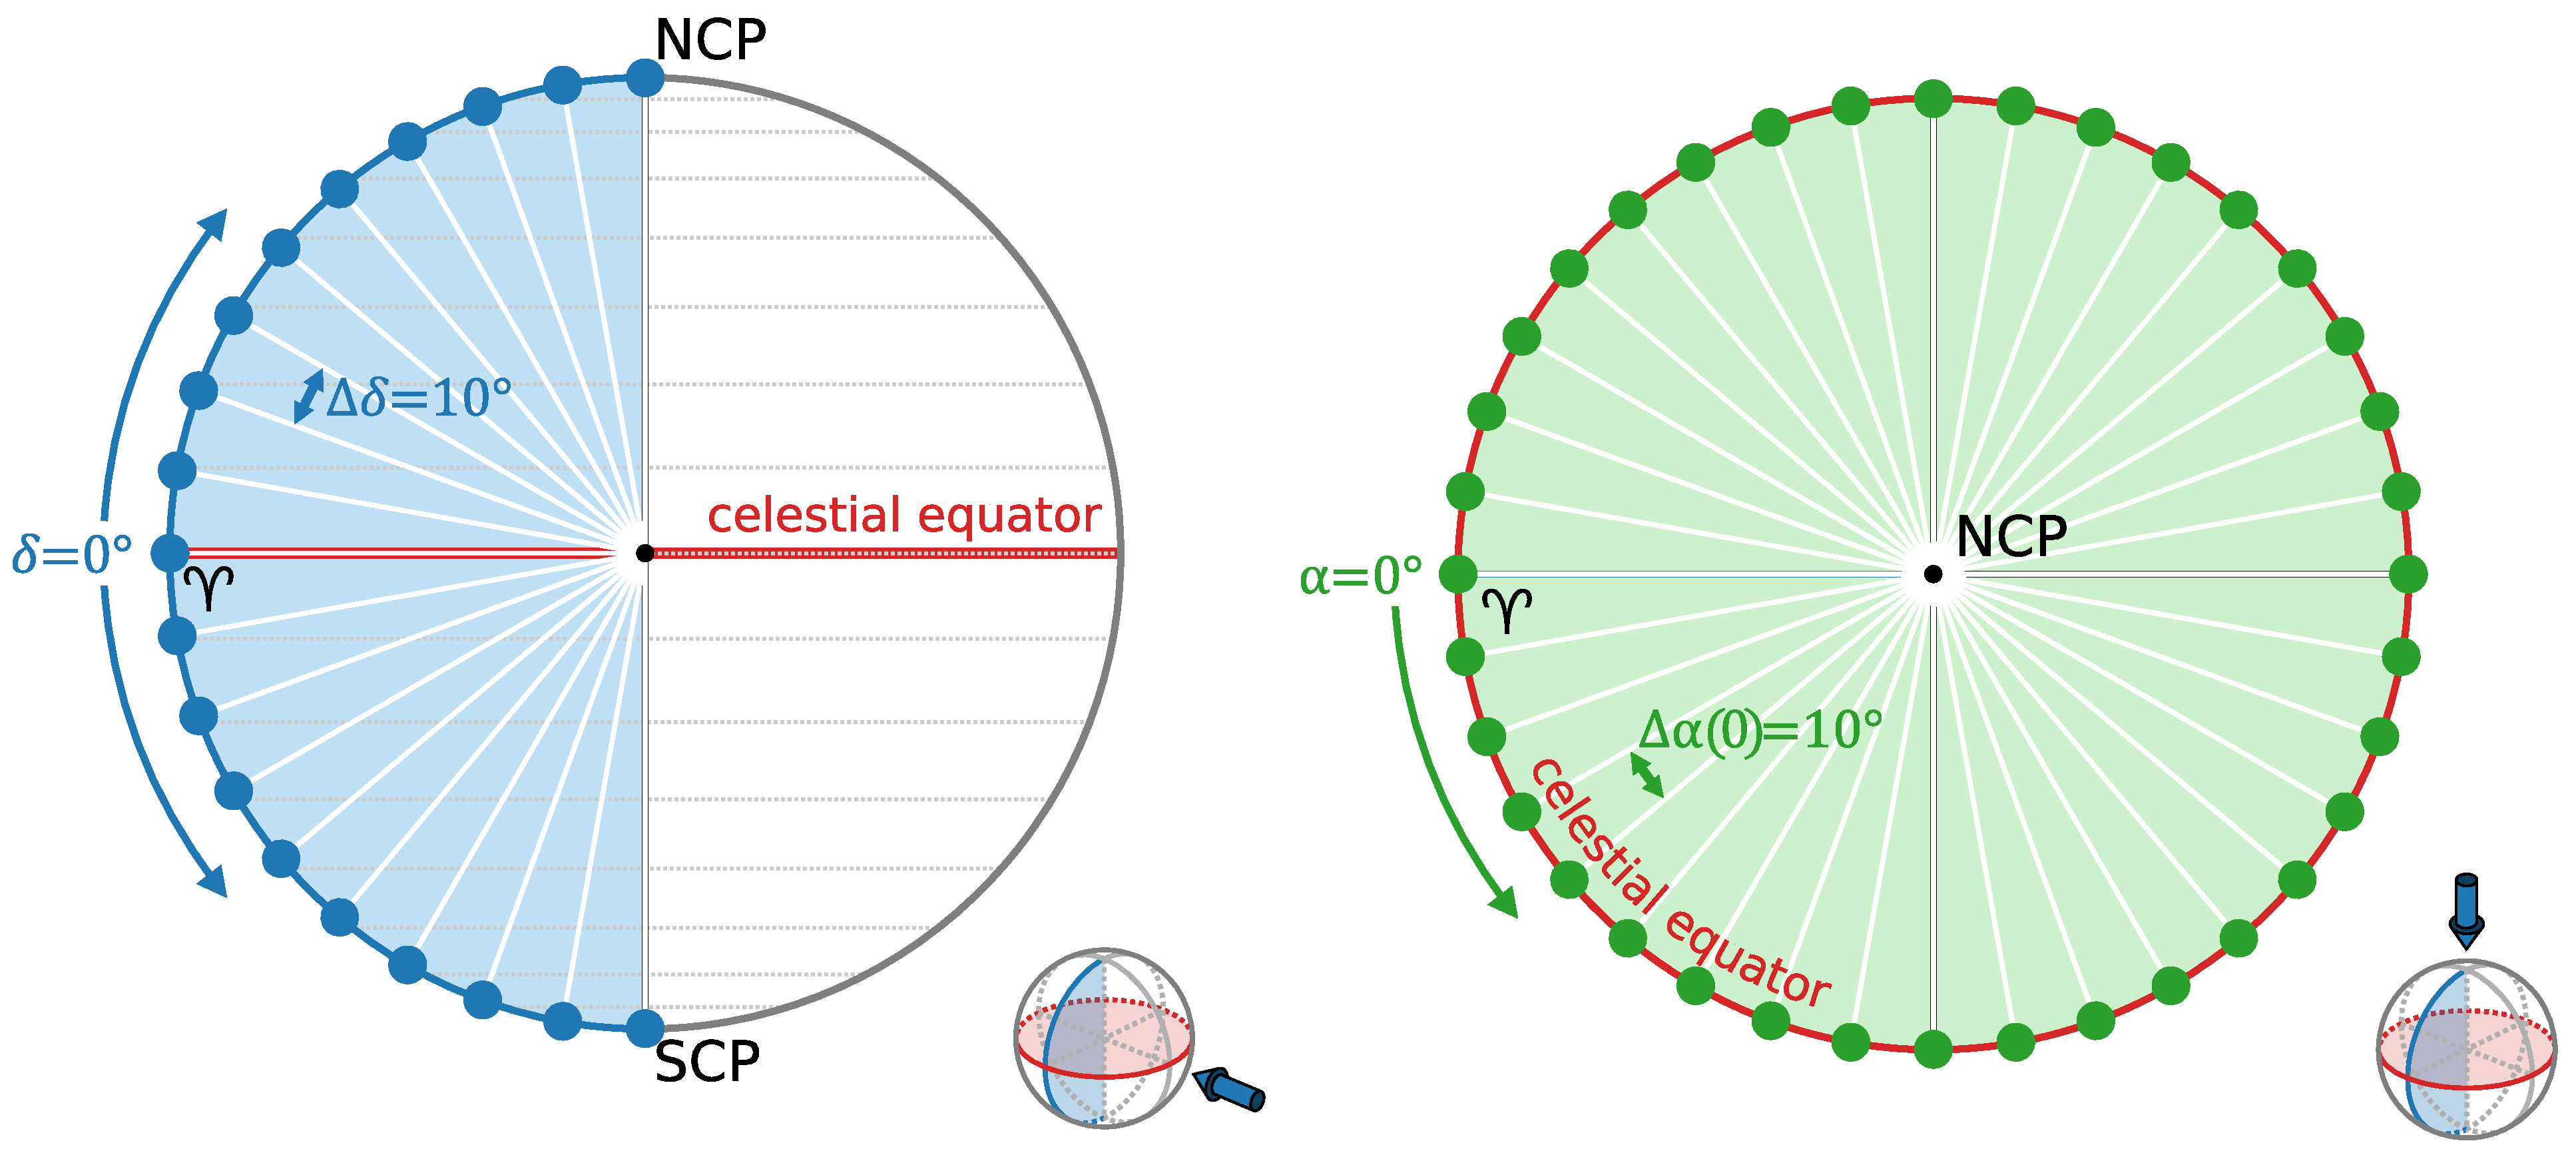
\includegraphics[width=\linewidth]{images/spacing_minverlap.pdf}
    \end{center}
    \caption[Grid spacing with the minverlap algorithm]{
        Grid spacing with the minverlap algorithm. Using the same parameters as \aref{fig:cosine_spacing} \aref{eq:minverlap_deltadelta} gives $\Delta\delta = $ \SI{10}{\degree}, therefore neatly arranging 19 declination strips between \SI{-90}{\degree} and \SI{90}{\degree}. \aref{eq:minverlap_deltaalpha} also gives $\Delta\alpha = $ \SI{10}{\degree} on the equator ($\delta=0$), so 36 points are uniformly arranged around the circumference.
    }\label{fig:minverlap_spacing}
\end{figure}

\clearpage

To define the grid points using the minverlap algorithm, it is first necessary to find the number of tiles $n$ that would fit into the available range using the cosine algorithm spacing; if this is not an integer number of tiles then round it up to the next whole number. In declination this is calculated as
%
\begin{equation}
    n_\text{dec} = \left \lceil \frac{90}{f_\text{dec}(1-v_\text{dec})} \right \rceil,
    \label{eq:minverlap_ndec}
\end{equation}
%
where $\lceil x \rceil$ is the mathematical ceiling function. This is a modification of \aref{eq:product_deltadelta}, but one that will always find an integer number of tiles. For example, for a tile with a declination field of view $f_\text{dec} = $ \SI{13}{\degree} and overlap $v_\text{dec} = 0.2$ \aref{eq:product_deltadelta} gives $\Delta\delta = 13 \times (1-0.2) = $ \SI{10.4}{\degree}. This clearly does not divide into \SI{90}{\degree} without a remainder, \SI{6.8}{\degree}, as shown in \aref{fig:cosine_spacing}. The problem is that \SI{90}{\degree} $/$ \SI{10.4}{\degree} $= 8.65$, so the product and cosine algorithms will fit in 8 declination strips and then have over half the height of a tile remaining at the poles. Instead, the minverlap algorithm rounds this up to $n_\text{dec} = 9$ and then calculates the spacing using
%
\begin{equation}
    \Delta\delta = \frac{90}{n_\text{dec}}.
    \label{eq:minverlap_deltadelta}
\end{equation}

In this case the new $\Delta\delta = $ \SI{10}{\degree}, which gives an even arrangement of tiles from the equator to the poles, as shown in \aref{fig:minverlap_spacing}. The other benefit of this method is that, in addition to there always being a declination strip at $\delta=0$, there will always be ``strips'' at \SI{+90}{\degree} and \SI{-90}{\degree}, which results in a single tile being located over the celestial poles and ensuring there are no major gaps in coverage.

In the minverlap algorithm the spacing in right ascension is treated in a simula way. The integer number of tiles that can fit into a given declination strip is given by
%
\begin{equation}
    n_\text{RA}(\delta) = \left \lceil \frac{360}{f_\text{RA}(1-v_\text{RA})/\cos \delta} \right \rceil + 1,
    \label{eq:minverlap_nra}
\end{equation}
%
where the $+1$ is  to account for tiles being located both at $\alpha=$\SI{0}{\degree} and $\alpha=$\SI{360}{\degree}. The logic is exactly the same as with declination, and the revised spacing is given by
%
\begin{equation}
    \Delta\alpha(\delta) = \frac{360}{n_\text{RA}(\delta)}.
    \label{eq:minverlap_deltaalpha}
\end{equation}

This spacing is also shown in \aref{fig:minverlap_spacing}, with the grid points uniformly spaced around the celestial equator. Note that the ceiling function does mean that in some cases strips at different declinations can have the same number of tiles. For example, using the same parameters as previously $\Delta\delta=$\SI{10}{\degree}, so declination strips start at \SI{0}{\degree} and continue to \SI{\pm10}{\degree}, \SI{\pm20}{\degree} \ldots (mirrored in both hemispheres). From \aref{eq:minverlap_nra} the number of tiles on the equator is $n_\text{RA}(\delta=\SI{0}{\degree}) = \lceil 360/(10.4/\cos \SI{0}{\degree}) \rceil + 1 = \lceil 34.6 \rceil + 1 = 36$. But on the next strip up (or down) $n_\text{RA}(\delta=\SI{\pm10}{\degree}) = \lceil 360/(10.4/\cos(\pm\SI{10}{\degree})) \rceil + 1 = \lceil 34.1 \rceil + 1 = 36$ as well. This occurs because there are only a limited number of ways to fit an integer number of fixed tiles into a given declination strip, and so, as shown in \aref{fig:minverlap}, the three strips around the equator align perfectly with the same number of tiles.

% ---------
\subsubsection{Limitations of the minverlap algorithm}

The new minverlap algorithm is a significant improvement on the previous gridding algorithms. In particular it reduces the occurrences of gaps in coverage close to the poles which occur when using the cosine algorithm. However gaps can still occur when using the minverlap with a particularly low overlap parameter. For example, \aref{fig:tiledsphere} shows a sphere tiled using the minverlap algorithm with an overlap parameter of 0 and in this case gaps are visible just below the northern celestial pole.

A proposed solution to this problem would be to force tiles to meet at their lower corners (in the northern hemisphere; upper corners in the south), therefore overlapping further and removing the possibility of gaps forming due to the angle between the tiles. An attempt to make this change and create an ``enhanced minverlap'' algorithm was tested, however ultimately it proved unnecessary. Although the current minverlap algorithm is deficient at low overlap values, this is only an issue when used with large tiles. The \SI{10}{\degree} $\times$ \SI{10}{\degree} tiles and 0 overlap used for \aref{fig:tiledsphere} are extreme values, and even for the roughly \SI{8}{\degree} $\times$ \SI{5}{\degree} full field of view of GOTO with 8 unit telescopes the overlap has to be less than 0.1 before noticeable gaps start appearing.

A further possible improvement to the minverlap algorithm has also been identified since it was implemented. Instead of locating two grid points precisely at the celestial poles (i.e.\ using declination strips at $\pm$\SI{90}{\degree}) as show in \aref{fig:minverlap_spacing}, it would instead be enough to have the highest/lowest declination strips exactly half of the field of view away from the poles. This would ensure the poles were still included within the tiled area, at the top/bottom of the highest/lowest strip, but could reduce the number of strips needed to cover the entire sphere.

As it happens, when viewed from La Palma, the northern celestial pole is below the GOTO altitude limit of \SI{30}{\degree}. This means that tiles closest to the pole are not visible, and so the issues described above are irrelevant. Should GOTO-tile be applied in the future to other telescopes at other sites then this issue would need to be revisited, but it was not a priority to fix within the context of this work.

\end{colsection}

% ~~~~~~~~~~~~~~~~~~~~

\end{colsection}

% ########################################

\newpage
\section{Probability skymaps}
\label{sec:skymaps}
\begin{colsection}

% ~~~~~~~~~~~~~~~~~~~~

\begin{colsection}

When identifying a particular target in the sky coordinates can be given in right ascension and declination, and if there is some uncertainty in the position then errors can be given on the coordinate values. For example, a \glsfirst{grb} event detected by the \textit{Fermi} \glsfirst{gbm} might have a central position and an error radius ranging from arcseconds to tens of degrees. However, multiple gravitational-wave detectors produce large and distinctly asymmetric localisation areas (see \aref{sec:gw_localisation}). For these cases, the \glsfirst{lvc} produce probability skymaps which map the localisation area onto the celestial sphere. This section describes how these skymaps are defined and how they are mapped onto the GOTO all-sky grid as described in \aref{sec:gototile}.

\end{colsection}

% ~~~~~~~~~~~~~~~~~~~~

\subsection{Defining skymaps with HEALPix}
\label{sec:healpix}
\begin{colsection}

\glsfirst{healpix} is a system used to define pixelised data on the surface of a sphere~\citep{HEALPix}. Developed at NASA JPL for microwave background data, it is now widely used for other applications including for gravitational-wave skymaps produced by the LVC.\@ HEALPix divides the sphere into a series of nested (hierarchical), equal-area (although not equal-shape) pixels arranged in declination strips (``isoLatitude''). The first four orders of spheres are shown in \aref{fig:healpix}, starting from a base resolution with 12 pixels and increasing as each pixel is split into four.

\begin{figure}[t]
    \begin{center}
        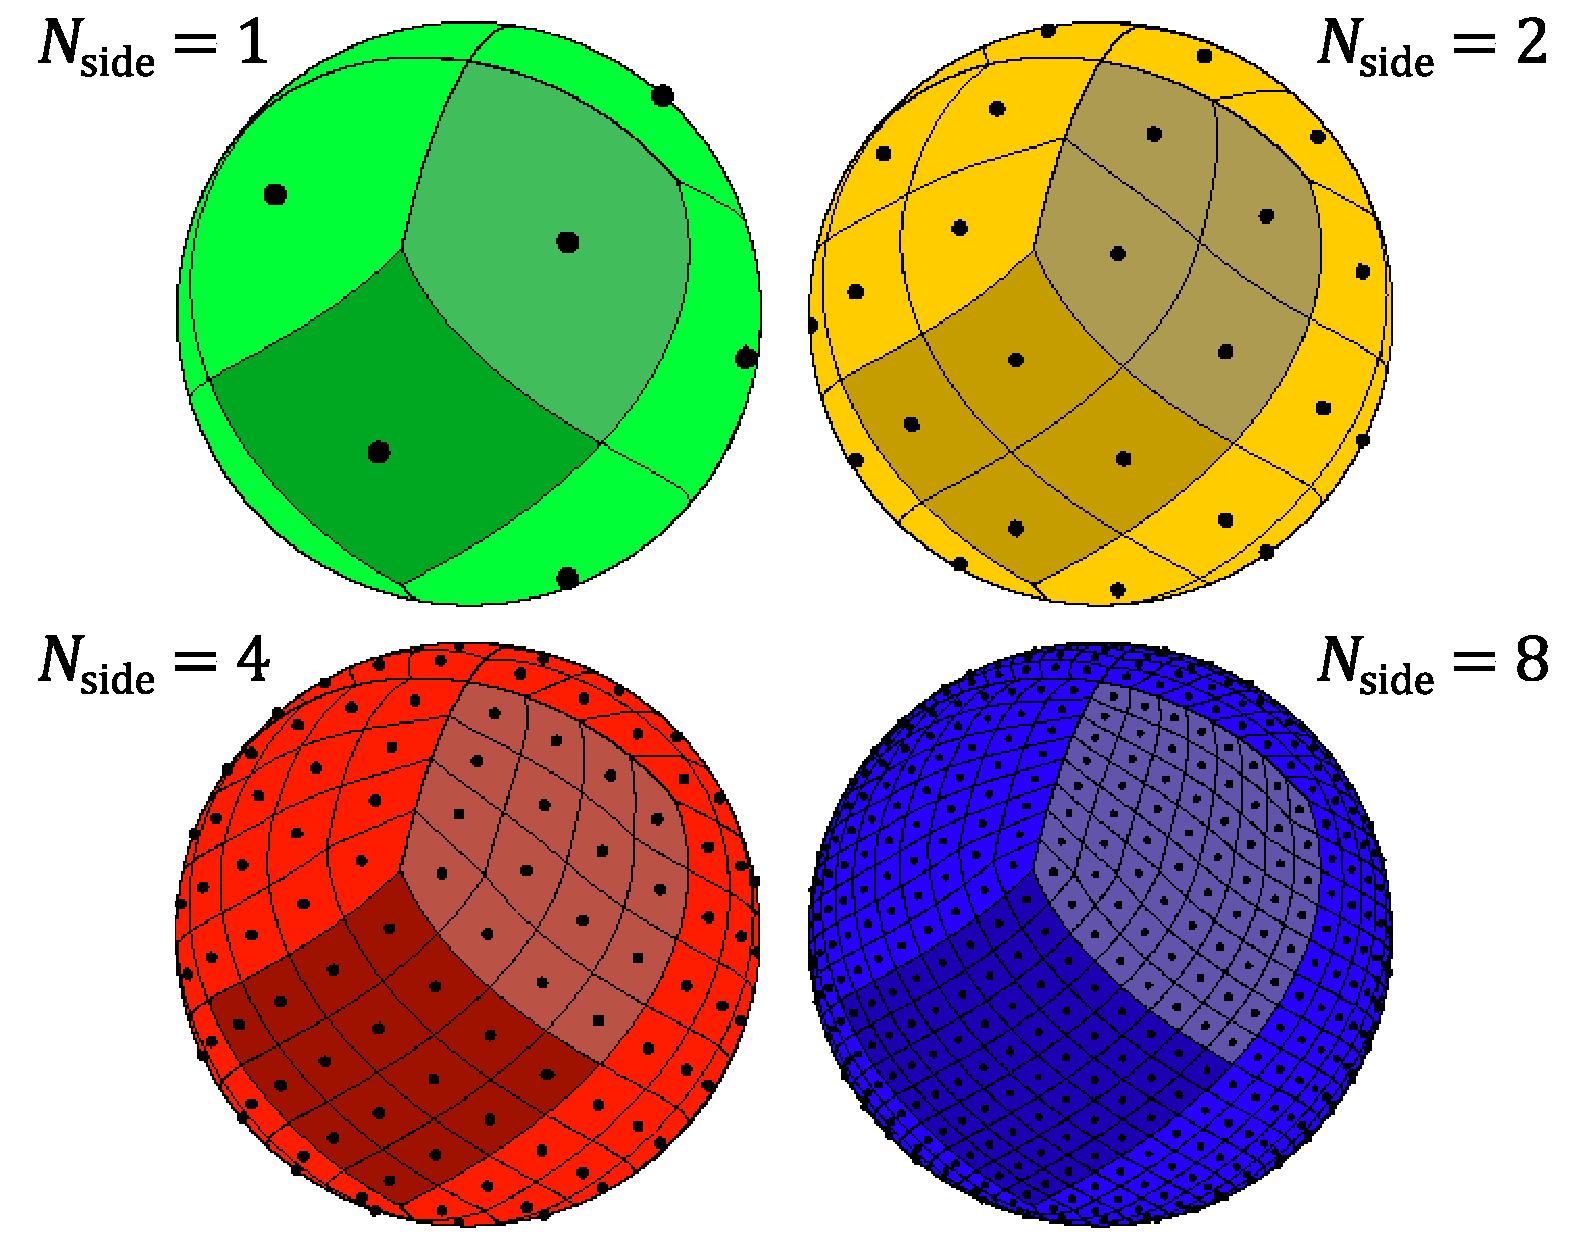
\includegraphics[width=0.7\linewidth]{images/healpix.pdf}
    \end{center}
    \caption[HEALPix partitions of a sphere]{
        The first four orders of the HEALPix partition of a sphere, with increasing $N_\text{side}$ resolution parameter. Note that as the resolution doubles each pixel on the previous sphere is split into four, and $N_\text{side}$ is the number of pixels along the side of a first-order pixel (two of which are highlighted). Adapted from \citet{HEALPix}.
    }\label{fig:healpix}
\end{figure}

The resolution of the HEALPix grid is defined using the $N_\text{side}$ parameter, which for the given resolution is the number of pixels along each side of one of the 12 base pixels. At every resolution each first-order pixel contains $N_\text{side}^2$ pixels, so the total number of pixels in a sphere is given by
%
\begin{equation}
    N_\text{pix} = 12 N_\text{side}^2.
    \label{eq:healpix_npix}
\end{equation}
%
Each pixel therefore has an equal area of
%
\begin{equation}
    \Omega_\text{pix} = \frac{4\pi}{12 N_\text{side}^2} = \frac{\pi}{3 N_\text{side}^2},
    \label{eq:healpix_area}
\end{equation}
%
on a unit sphere where the radius $r=1$. Taking the celestial sphere, the circumference in degrees is $\SI{360}{\degree} = 2 \pi r$ meaning the area of the whole sky is given by
%
\begin{equation}
    A_\text{sky} = 4 \pi r^2 = 4 \pi \left ( \frac{\SI{360}{\degree}}{2 \pi} \right )^2 = \frac{129600}{\pi}~\text{sq deg} \approx 41252~\text{sq deg} , %chktex 3
    \label{eq:sky_area}
\end{equation}
%
and therefore the area of each HEALPix pixel is
%
\begin{equation}
    A_\text{pix} = \frac{129600}{12 \pi N_\text{side}^2}~\text{sq~deg} \approx \frac{3438}{N_\text{side}^2}~\text{sq~deg}.
    \label{eq:healpix_area_degrees}
\end{equation}

\aref{fig:healpix} shows only the first four orders of HEALPix pixelisation, up to $N_\text{side} = 8$ where the sphere is split into 768 pixels each with an area of 53.7~sq deg. An initial, low-resolution LVC skymap might use a grid with $N_\text{side} = 64$ (approximately 49 thousand pixels) and each with an area of 0.84~sq~deg, whereas a final output skymap will have $N_\text{side} = 1024$, 12.5 million pixels and a pixel size resolution of $3.27 \times 10^{-3}$~sq~deg (11.7~square~arcminutes).

In addition to being a way to divide the sphere, each HEALPix pixel has a unique index from one of two different numbering schemes: either the ring (counting around each ring from the north to the south) or nested (based on the sub-pixel tree) system.

HEALPix is used to provide localisation of sky probabilities for transient astronomical events, in the form of ``skymaps''. Each point on the HEALPix grid is assigned a probability between 0 and 1 that the counterpart object is located within that pixel, and the whole sphere should sum to unity. \aref{fig:skymap_regrade} shows a typical LVC skymap, for the gravitational-wave event S190521r \citep{S190521r}, at various HEALPix $N_\text{side}$ parameters.

\begin{figure}[p]
    \begin{center}
        \begin{tabular}{cc}
            $N_\text{side} = 1$: &
            $N_\text{side} = 2$: \\
            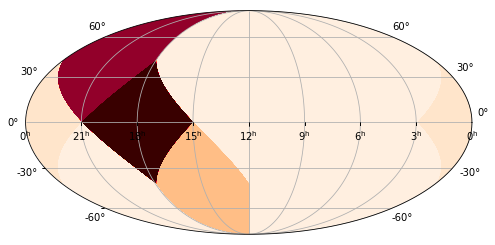
\includegraphics[width=0.45\linewidth]{images/regrade/1.png} &
            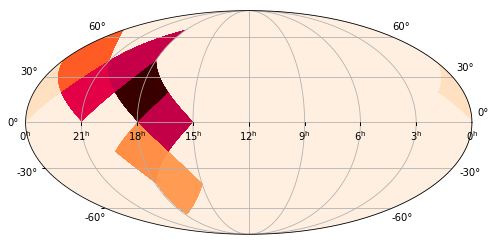
\includegraphics[width=0.45\linewidth]{images/regrade/2.png} \\
            \\
            $N_\text{side} = 4$: &
            $N_\text{side} = 8$: \\
            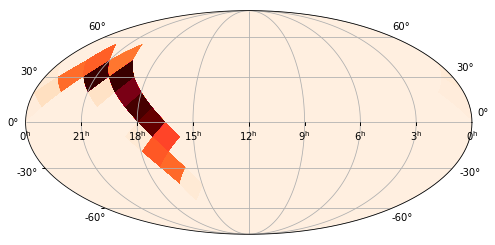
\includegraphics[width=0.45\linewidth]{images/regrade/4.png} &
            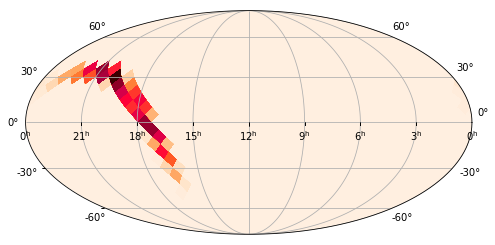
\includegraphics[width=0.45\linewidth]{images/regrade/8.png} \\
            \\
            $N_\text{side} = 16$: &
            $N_\text{side} = 32$: \\
            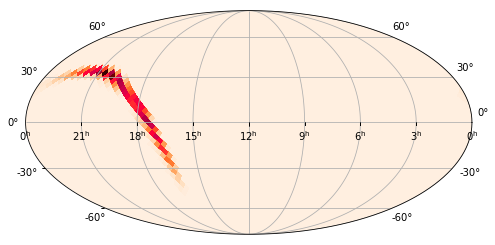
\includegraphics[width=0.45\linewidth]{images/regrade/16.png} &
            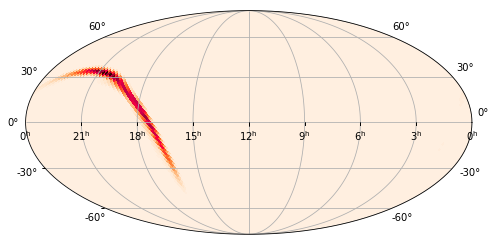
\includegraphics[width=0.45\linewidth]{images/regrade/32.png} \\
            \\
            $N_\text{side} = 64$: &
            $N_\text{side} = 128$: \\
            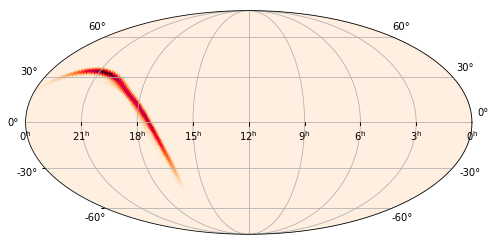
\includegraphics[width=0.45\linewidth]{images/regrade/64.png} &
            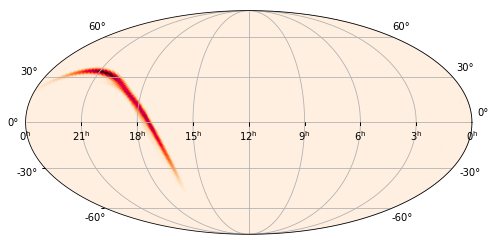
\includegraphics[width=0.45\linewidth]{images/regrade/128.png} \\
        \end{tabular}
    \end{center}
    \caption[Regrading a gravitational-wave skymap]{
        Changing the HEALPix resolution of a gravitational-wave skymap (also known as regrading). At every stage each pixel is assigned a probability value which indicates the probability the source is located within that pixel, here darker colours denote higher probabilities. At lower $N_\text{side}$ values individual pixels are visible, but as the resolution increases the HEALPix structure is less visible.
    }\label{fig:skymap_regrade}
\end{figure}

As well as the individual probabilities assigned to each pixel, it is also useful to consider the overall spread of the probability. This is done by considering the probability contour areas, typically at the 50\% and 90\% levels. The 50\% contour area of a skymap is defined by encircling the smallest number of pixels so that the total probability within the area is 50\% of the overall skymap probability. When a skymap is processed using GOTO-tile each pixel is assigned a contour value as well as its individual probability value. This is calculated by sorting all of the pixels by probability from highest to lowest, and the contour value for each pixel is then the cumulative sum of the probability within the pixels above it. This contour value can be considered as the lowest contour area that each pixel is within, meaning the pixels that are contained within the 50\% contour area are those with contour values of less than 50\%. \aref{fig:sim_skymap_probs} and \aref{fig:sim_skymap_conts} illustrate how the contours are calculated for a cartoon 2-dimensional skymap.

\makeatletter
\setlength{\@fptop}{1cm}
\makeatother

\begin{figure}[t]
    \begin{center}
        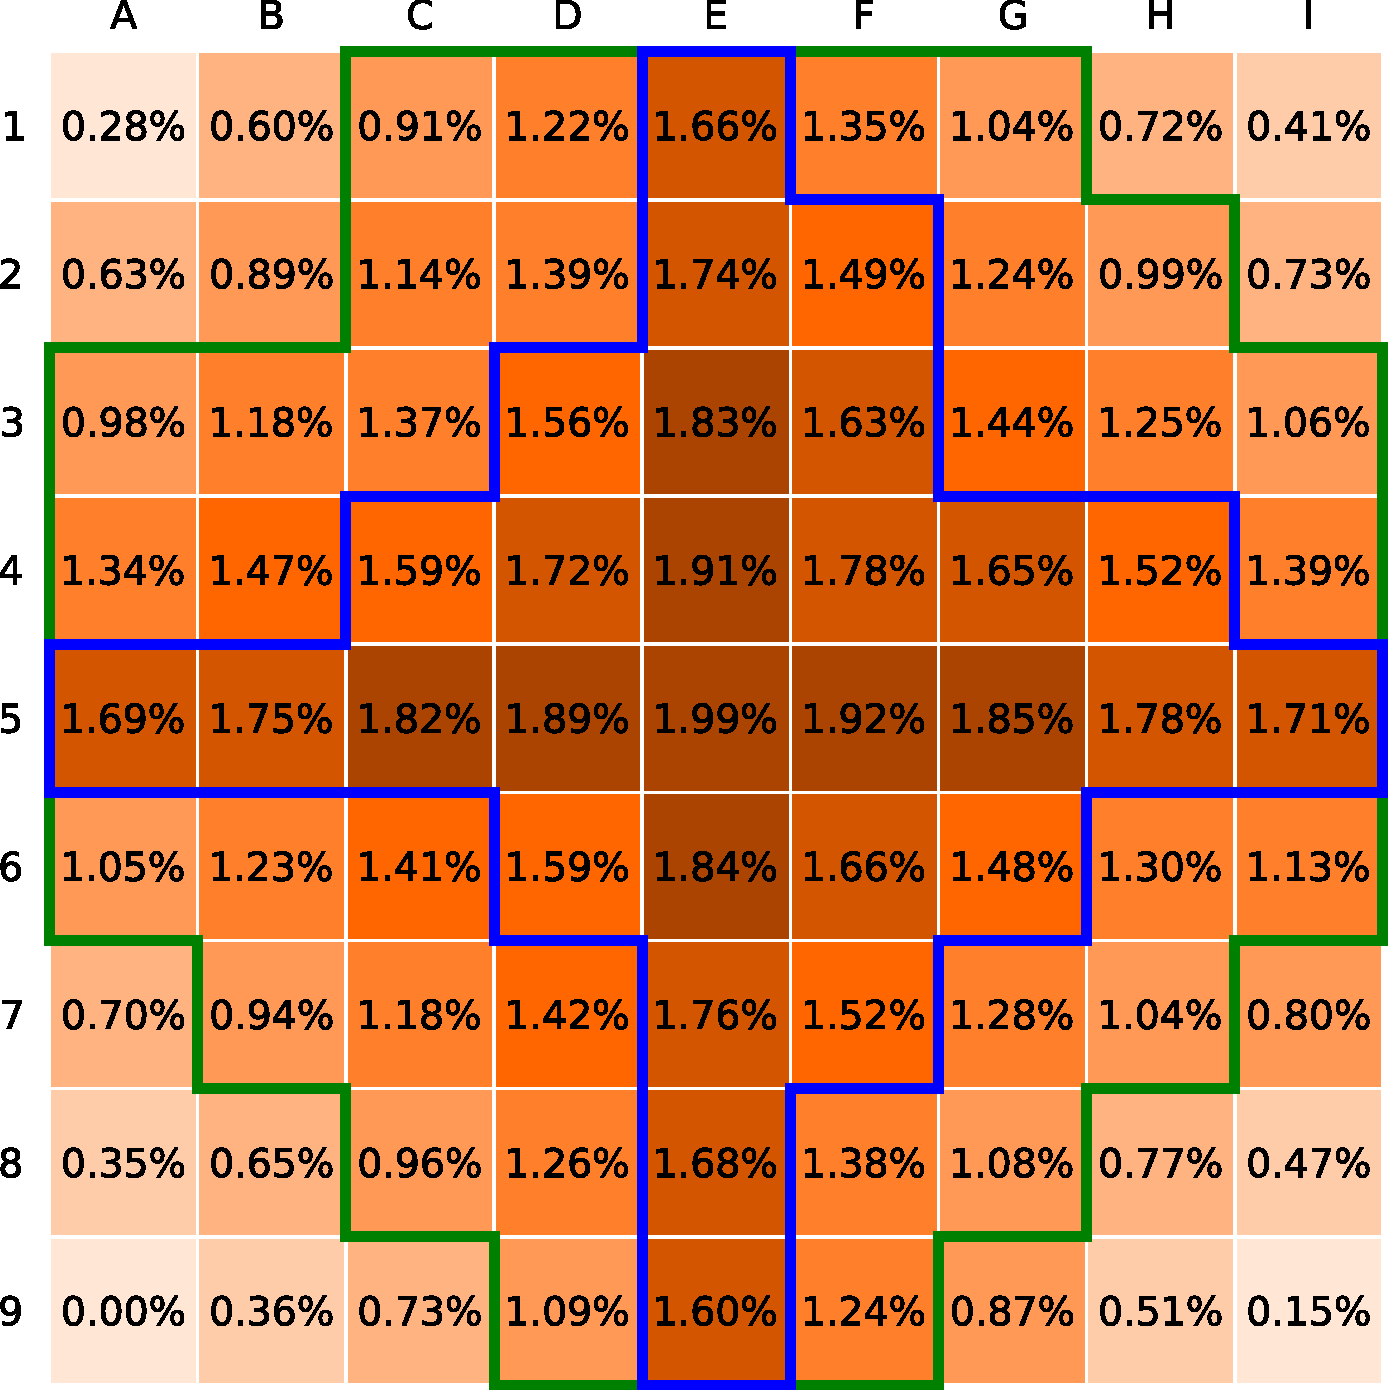
\includegraphics[width=0.95\linewidth]{images/sim/sim_skymap_probs.pdf}
    \end{center}
    \caption[An example 2D probability skymap]{
        A cartoon 2-dimensional skymap. Each pixel (represented by one of the 81 squares) has an assigned probability, and together they all sum to 100\%. The \textcolorbf{BlueGreen}{blue} inner contour contains 50\% of the probability, while the \textcolorbf{Green}{green} outer contour contains 90\% of the probability. These contours are created based on the values shown in \aref{fig:sim_skymap_conts}.
    }\label{fig:sim_skymap_probs}
\end{figure}

\clearpage

\begin{figure}[t]
    \begin{center}
        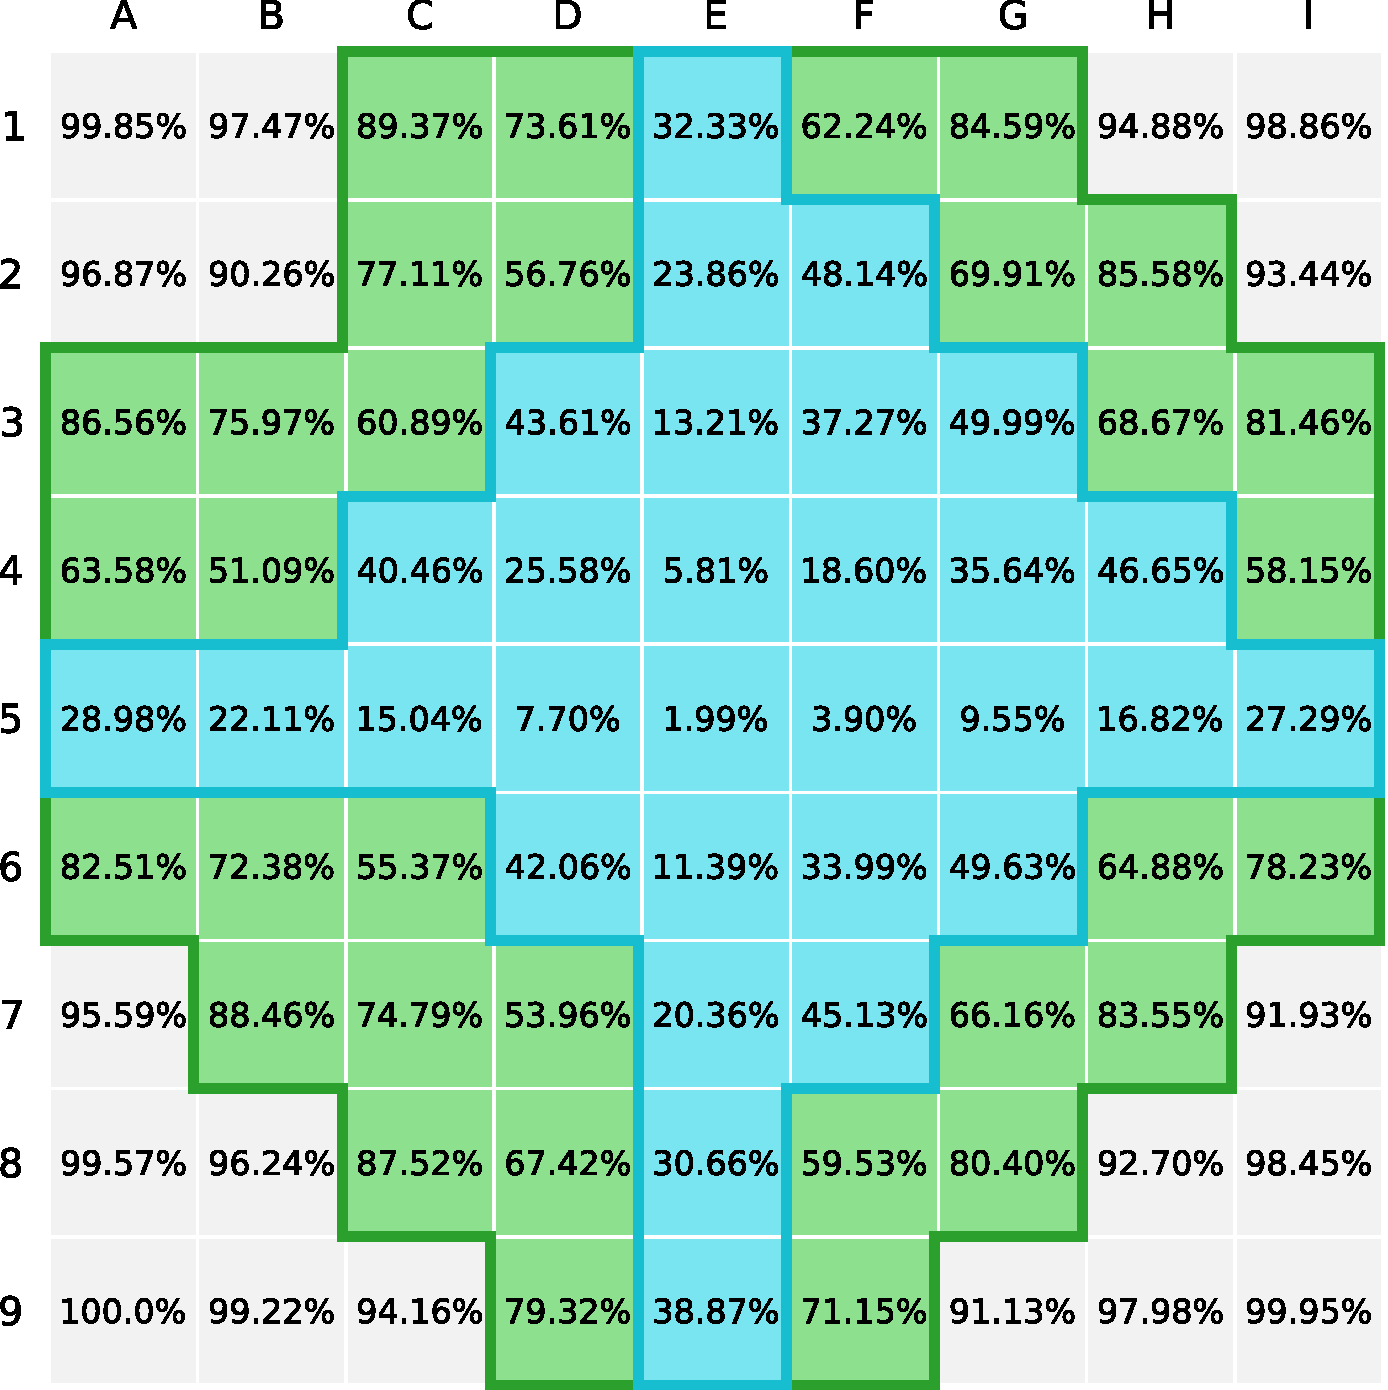
\includegraphics[width=0.95\linewidth]{images/sim/sim_skymap_conts.pdf}
    \end{center}
    \caption[An example 2D skymap with pixel contour values]{
        The same cartoon skymap as in \aref{fig:sim_skymap_probs}, but now each pixel contains its contour value calculated by sorting the pixels by probability and assigning each pixel the value of the cumulative sum. The pixel with the highest probability (E5) has the same contour value as its probability value, the second highest (F5) has the sum of the probability values of both E5 and F5, and this continues to the pixel with the lowest probability value (A9) which has a contour value of 100\%. The \textcolorbf{BlueGreen}{blue} area is the 50\% probability contour, which encloses all pixels with a contour value of less than 50\%. The \textcolorbf{Green}{green} area likewise encloses all pixels with a contour value of less than 90\%. Note in this example the contours are continuous, but it is possible to have multiple `islands' of probability within a single skymap.
    }\label{fig:sim_skymap_conts}
\end{figure}

\clearpage

\makeatletter
\setlength{\@fptop}{0\p@ \@plus 1fil} % chktex 1
\makeatother

\end{colsection}

% ~~~~~~~~~~~~~~~~~~~~

\newpage
\subsection{Mapping skymaps onto the grid}
\label{sec:mapping_skymaps}
\begin{colsection}

When gravitational-wave signals are detected the LVC analysis pipelines create HEALPix skymaps to describe the sky localisation, and these are then distributed with the public VOEvent (see \aref{sec:voevents}). GOTO-tile is used to map the skymaps onto the grid used for the all-sky survey (defined in \aref{sec:gototile}). This requires finding which HEALPix pixels fall within each tile, which is done by defining polygons that match the projected tile areas and using the \code{query\_polygon} function from the healpy Python package (\pkg{healpy}\footnote{\url{https://healpy.readthedocs.io}}). For each tile it is then simple to sum the probability of all the HEALPix pixels within it, which gives the total contained probability. This is shown for a cartoon skymap in \aref{fig:sim_skymap_tiles}. In cases where grid tiles overlap a given HEALPix pixel could fall within the area of multiple tiles, and therefore that pixel would contribute to the total probability of more than one tile. This means the total contained probability within all tiles can add to more than 100\%.

\begin{figure}[t]
    \begin{center}
        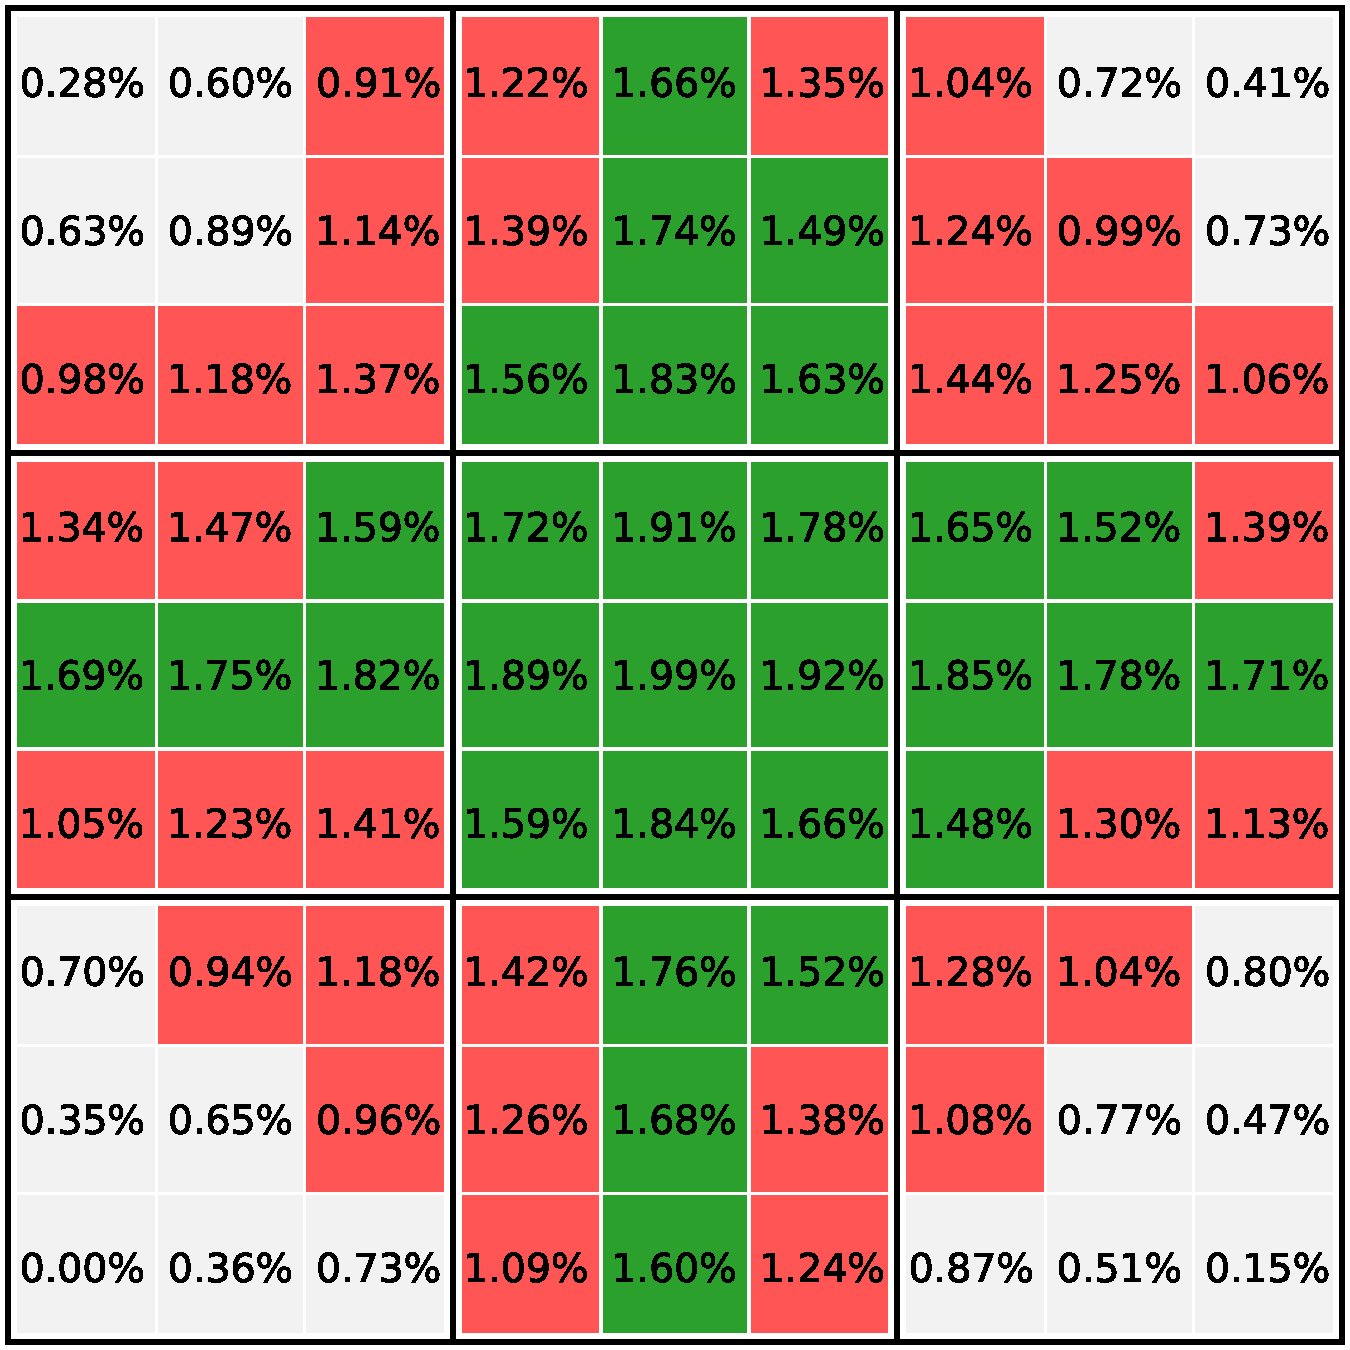
\includegraphics[width=0.46\linewidth]{images/sim/sim_skymap_pix_probs.pdf}
        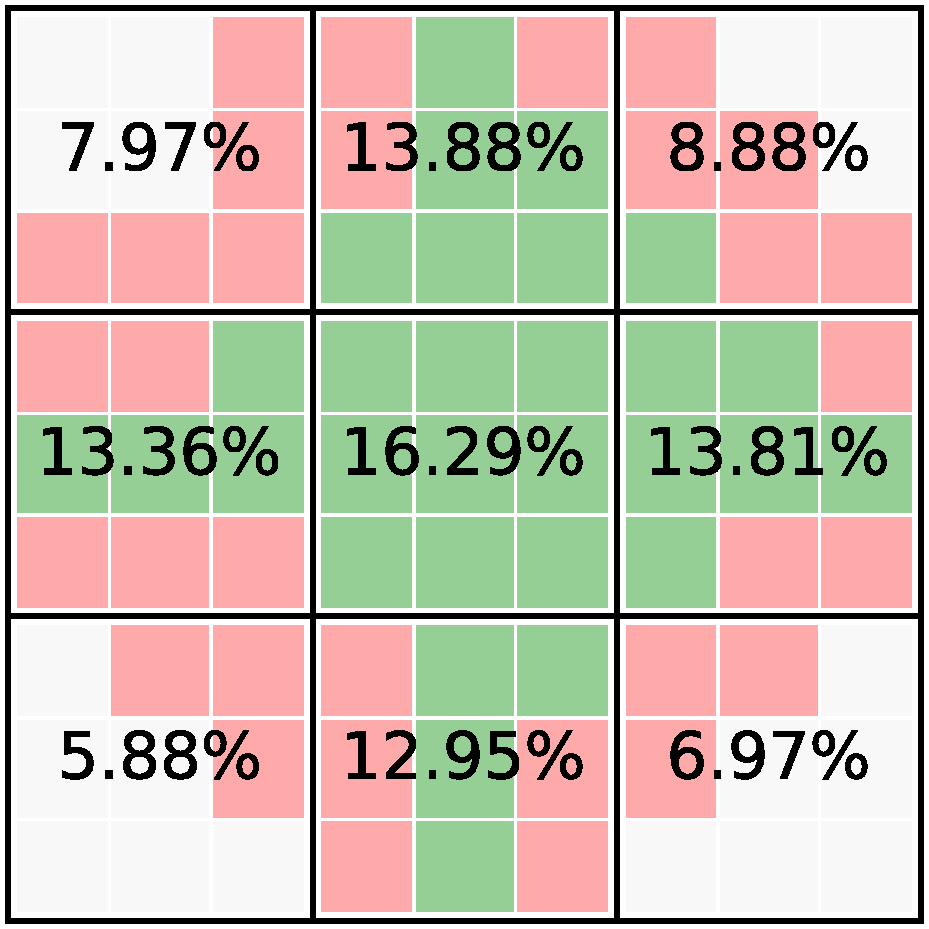
\includegraphics[width=0.46\linewidth]{images/sim/sim_skymap_tile_probs.pdf}
    \end{center}
    \caption[Mapping a 2D probability skymap onto grid tiles]{
        On the left, the cartoon skymap from \aref{fig:sim_skymap_probs} has been divided into nine survey grid tiles (outlined in \textcolorbf{Red}{red}). On the right, the total contained probability for each tile is found by summing the probability of nine pixels within them.
    }\label{fig:sim_skymap_tiles}
\end{figure}

\end{colsection}

% ~~~~~~~~~~~~~~~~~~~~

\newpage
\subsection{Selecting tiles}
\label{sec:selecting_tiles}
\begin{colsection}

When a gravitational-wave event is processed event pointings are added into the observation database as described in \aref{sec:event_insert}. However, only a certain number of pointings should be added to prevent GOTO wasting too much time observing low-probability areas. Each pointing is mapped to a grid tile, and only tiles with a reasonably high contained probability are worth observing. The GOTO-alert event handling code described in \aref{chap:alerts} selects tiles based on their contour level, meaning GOTO could, for example, chose to observe the 90\% contour of each skymap. However, determining which contour level each tile is within is not as simple as calculating the contained probability, as there are multiple ways to define the contour value for each tile.

For example, a tile could be defined as being within a given contour area if \textit{every} pixel contained within that tile is within that contour. However this is unreasonable for large tiles, such as GOTO's, as the tile areas are often wider than the long, stretched out probability areas seen in typical gravitational-wave typical skymaps. An alternative then would be say that a tile is within a contour if \textit{any} of its contained pixels are within the contour. However, this will find every tile covering the contour area even if only the smallest fraction of the tile's area is within that region, which leads to over-selecting tiles. Several alternative methods were considered, including taking the median or mean of the contained pixel contour levels within each tile. Some different selection methods applied to the S190521r skymap are shown in \aref{fig:selecting_tiles}.

The method used within the GOTO-alert event handler is to select all tiles which have a mean contour value within 90\%. However, more quantitative simulations of different skymaps could be used to determine if this is the optimal choice for all cases. For example, the selection level could be modified depending on the size of the skymap, and the event strategy might need to be modified as more GOTO telescopes are built. These possibilities are discussed in \aref{sec:event_insert}.

\begin{figure}[p]
    \begin{center}
        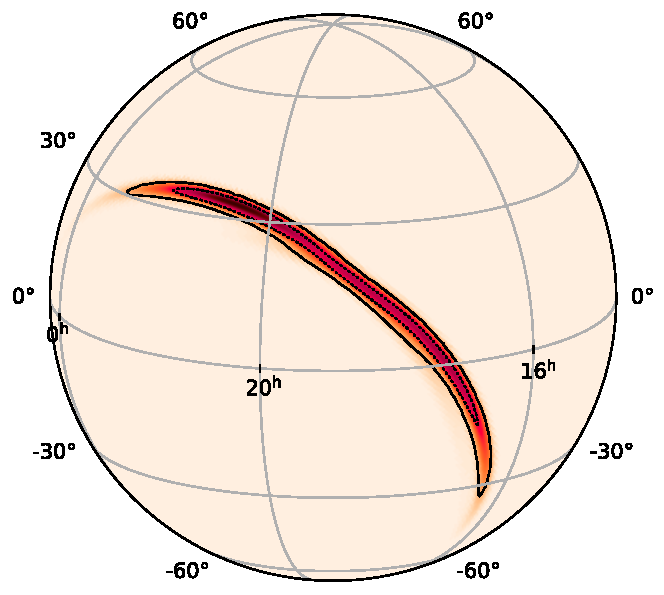
\includegraphics[width=0.49\linewidth]{images/tiling/S190521r_1.pdf}
        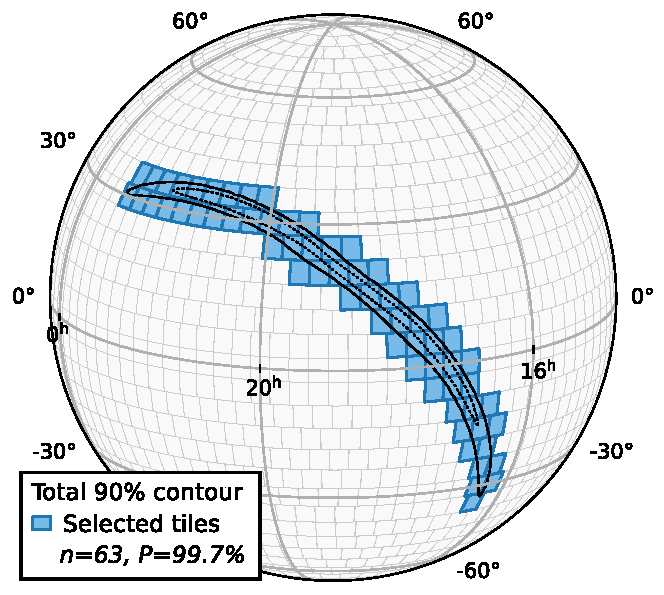
\includegraphics[width=0.49\linewidth]{images/tiling/S190521r_2.pdf}

        \vspace{0.5cm}

        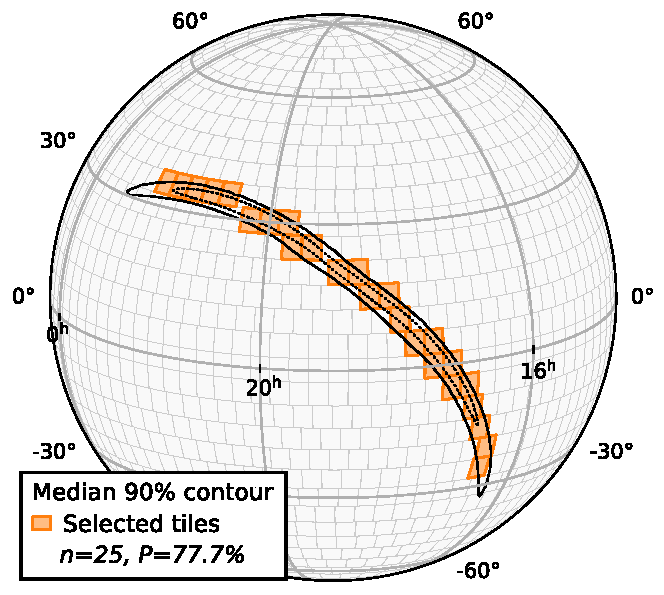
\includegraphics[width=0.49\linewidth]{images/tiling/S190521r_3.pdf}
        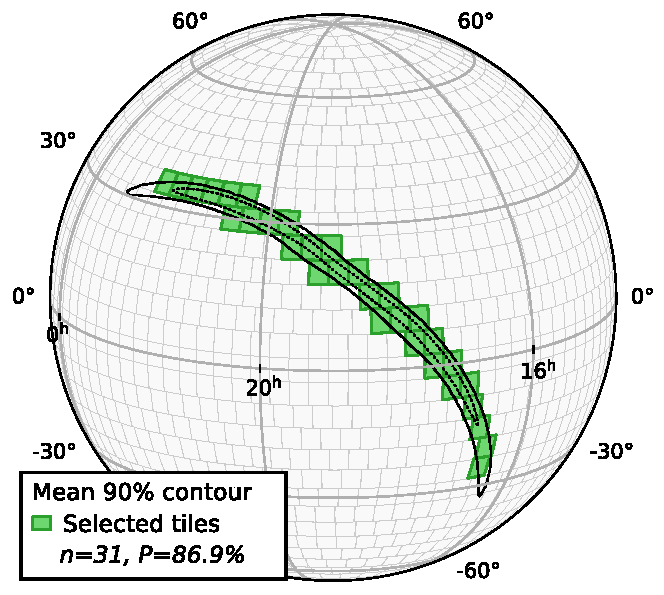
\includegraphics[width=0.49\linewidth]{images/tiling/S190521r_4.pdf}
    \end{center}
    \caption[Selecting tiles for a gravitational-wave skymap]{
        Selecting tiles for the S190521r skymap \citep[also shown in \aref{fig:skymap_regrade}]{S190521r}.
        In the upper left the skymap is plotted on the celestial sphere, forming the ``banana'' shape typical of gravitational-wave localisations, and the 50\% and 90\% probability contours are shown.
        The other three plots show grid tiles selected using one of three methods: selecting tiles to cover the entire 90\% skymap (\textcolorbf{NavyBlue}{blue}), selecting tiles with a median contour value of 90\% (\textcolorbf{Orange}{orange}) and selecting tiles with a mean contour value of 90\% (\textcolorbf{Green}{green}). The number of tiles selected ($n$) and total probability within them ($P$) is given.
        The mean contour method provides a good compromise, selecting fewer than half of the tiles needed to cover the whole 90\% contour (31 compared to 63), but together they still contain nearly 87\% of the total probability.
    }\label{fig:selecting_tiles}
\end{figure}

\newpage

\begin{figure}[t]
    \begin{center}
        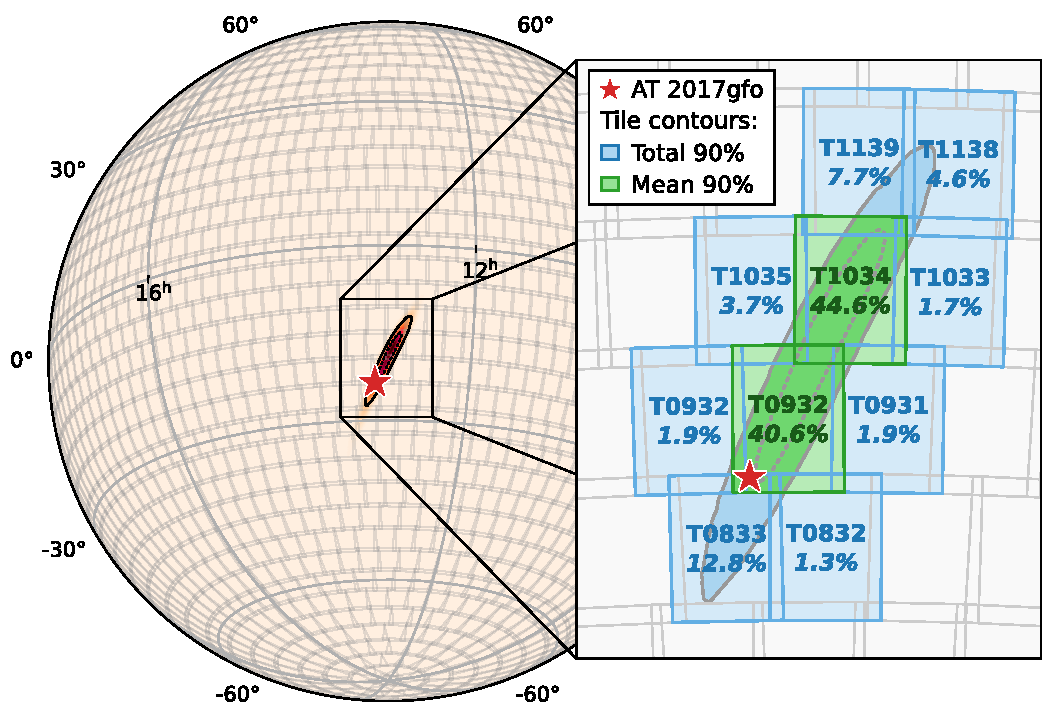
\includegraphics[width=\linewidth]{images/tiling/170817.pdf}
    \end{center}
    \caption[GOTO tile probabilities for GW170817]{
        GOTO tiling applied to the final GW170817 skymap \citep{GW170817}.
        The grid shown is for the 4-UT GOTO field of view, with tiles of \SI{3.7}{\degree}$\times$\SI{4.9}{\degree} and an overlap of $0.1$. The inset shows the 10 tiles within the total 90\% contour (containing 97.4\% of the total probability) in \textcolorbf{NavyBlue}{blue} and the 2 selected by the 90\% mean contour (containing 79.5\%) in \textcolorbf{Green}{green}. Compare to \aref{fig:swope_decam}, which shows follow-up observations of GW170817 by the Swope and DECam projects.
    }\label{fig:170817_gw}
\end{figure}

\aref{fig:170817_gw} shows the GOTO-tile selection code applied to the skymap for GW170817 \citep{GW170817}. As described in \aref{sec:followup} this is the only gravitational-wave detection so far with an identified counterpart, AT~2017gfo \citep{GW170817_followup}. In this case the mean contour selection method is perhaps too restrictive, only adding two tiles to the database, and for similarly well-localised events adding more tiles would be better. Still, based on the performance during commissioning (see \aref{sec:gw_results}) had GOTO been able to observe this event then the counterpart could have been observed in tile T0932 within minutes of the alert notice being received.

\end{colsection}

% ~~~~~~~~~~~~~~~~~~~~

\end{colsection}

% ########################################

\newpage
\section{Creating and modifying skymaps}
\label{sec:custom_skymaps}
\begin{colsection}

% ~~~~~~~~~~~~~~~~~~~~

\begin{colsection}

The GOTO-tile skymap processing system described in \aref{sec:skymaps} provides a working framework which allows any gravitational-wave skymap to be mapped onto the GOTO survey grid, from which pointings can be generated for the pilot to observe. However, there is no particular reason that the system has to be restricted to just the gravitational-wave skymaps produced by the LVC.\@ This section describes three further projects based on the GOTO-tile skymap code, from when I was working with Yik Lun Mong at Monash.

\end{colsection}

% ~~~~~~~~~~~~~~~~~~~~

\subsection{Creating Gaussian skymaps for GRB events}
\label{sec:grb_skymaps}
\begin{colsection}

As part of the GOTO commissioning observations when the LIGO-Virgo detectors were not operating (see \aref{sec:timeline}) GOTO followed up \glsfirst{grb} events from the \textit{Fermi} satellite Gamma-ray Burst Monitor \citep[GBM;][]{Fermi_GBM}. At the time the alert notices for GBM events did not include probability skymaps, only right ascension, declination and an error radius, and so code was developed in order to create a skymap from these details based on a 2D Gaussian profile; therefore allowing them to be processed by GOTO-tile using the same methods already created for gravitational-wave events.

Taking the radius $r$ as half the full-width at half-maximum, the standard deviation of a 2D Gaussian distribution $\sigma$ is given by
%
\begin{equation}
    \sigma = \frac{r}{\sqrt{2 \ln 2}}.
    \label{eq:gaussian_sigma}
\end{equation}
%
The distance $d$ between a given point on the sphere ($\alpha, \delta$) and the central coordinates of the distribution ($\alpha_c, \delta_c$) is given by
%
\begin{equation}
    \sin^2 \left ( \frac{1}{2} d \right )
    = \sin^2 \left ( \frac{\delta-\delta_c}{2} \right)
      + \cos \delta \cos \delta_c \sin^2 \left ( \frac{\alpha-\alpha_c}{2} \right),
    \label{eq:gaussian_distance}
\end{equation}

\noindent and the probability at each point is given by
%
\begin{equation}
    P(\alpha, \delta) = \frac{1}{2\pi\sigma} \exp \left ( \frac{d^2}{2\sigma^2} \right ).
    \label{eq:gaussian_prob}
\end{equation}
%
This probability is calculated for the location of every HEALPix pixel on a sphere, which produces a skymap array that can then be processed using GOTO-tile.

Using the above method, skymaps can be created for any single-target alert that has a given error radius. Several sources of transient events, such as \textit{Gaia} and \textit{Swift}, produce well-localised events with error circles much smaller than the GOTO tiles, so creating skymaps is less important. \textit{Fermi} GRB skymaps however cover much larger areas. For example, the GBM detection of GRB~170817A that helped localise the GW170817 gravitational-wave detection produced an initial alert with an error radius of \SI{17.45}{\degree}, later reduced to \SI{11.58}{\degree} in the final alert\footnote{GCN Notices available at \url{https://gcn.gsfc.nasa.gov/other/524666471.fermi}}, which corresponded to a 50\% confidence region of $\sim$500~square~degrees \citep{GW170817_Fermi}.

The error values given in GBM notices only account for statistical errors for that event, not systematic errors. The GBM systematic errors are described in \citet{Fermi_localisation} to be well modelled by a core Gaussian with a radius (FWHM) of \SI{3.71}{\degree} and a non-Gaussian tail extending to \SI{14}{\degree}. For the purposes of GOTO tiling the tail is ignored, and a single Gaussian is produced with a radius obtained by combining the statistical radius ($r_\text{notice}$) and the systematic error in quadrature as
%
\begin{equation}
    r = \sqrt{r_\text{notice}^2 + {(\SI{3.71}{\degree})}^2}.
    \label{eq:fermi_radius}
\end{equation}
%
This is then used with the previous method to create a Gaussian skymap, which can be processed by GOTO-tile as described in \aref{sec:mapping_skymaps}. The skymap generated using this method for GRB~170817A is shown in \aref{fig:170817_grb}. Note that the location of AT~2019gfo falls quite far from the reported peak of the GRB skymap, and had there not been the coincident gravitational-wave detection it would have been unlikely that the source of the gamma-ray burst would have been observed.

\begin{figure}[t]
    \begin{center}
        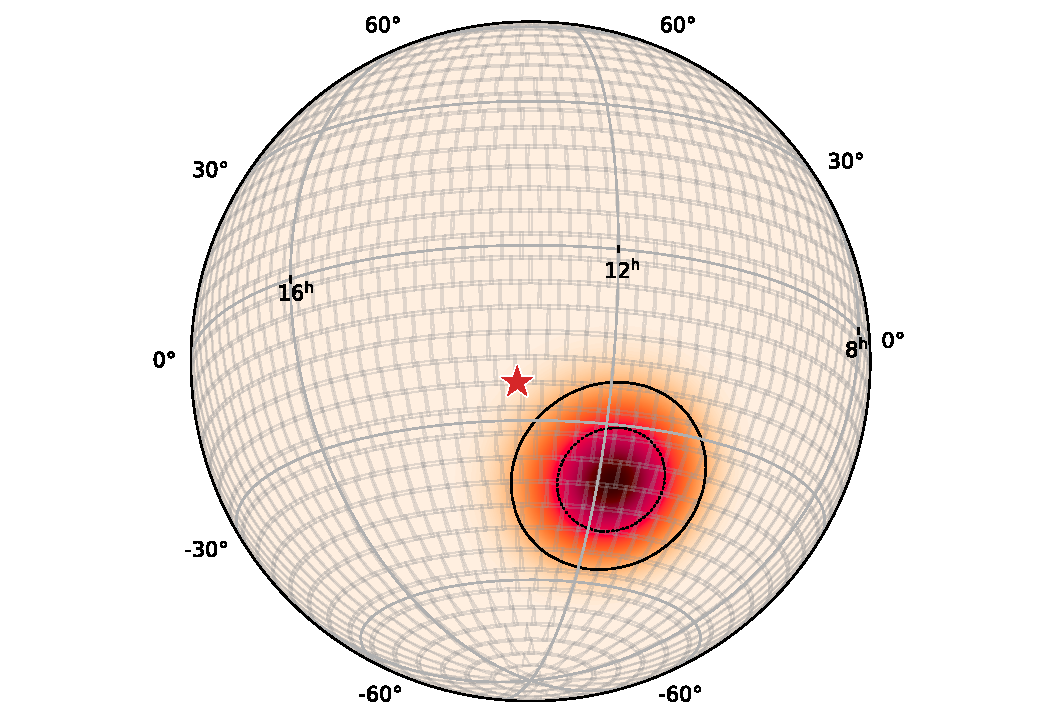
\includegraphics[width=\linewidth]{images/tiling/170817_fermi.pdf}
    \end{center}
    \caption[Gaussian skymap for GRB 170817A]{
        A Gaussian skymap generated from the initial GBM alert for GRB 170817A, shown on the GOTO tile grid. The \textcolorbf{Red}{red} star shows the location of the counterpart AT 2019gfo. The final GRB skymap for this event is shown in \aref{fig:170817_skymaps}.
    }\label{fig:170817_grb}
\end{figure}

It should be noted that the GBM localisation areas are actually not perfectly symmetric, but the above procedure works as a reasonable approximation. Since May 2019 \textit{Fermi} has started including HEALPix skymaps with alert notices \citep{Fermi_skymaps}, however, unlike the LVC, the GBM team do not guarantee that the skymap will have been generated by the time the alert notice is issued. Therefore the above procedure is still used when processing alerts if the official skymap is not yet available.

\end{colsection}

% ~~~~~~~~~~~~~~~~~~~~
\newpage
\subsection{Weighting GW skymaps using galaxy positions}
\label{sec:galaxy_skymaps}
\begin{colsection}

As described in \aref{sec:followup}, telescopes with much smaller fields of view than GOTO are not be able to cover the entirety of large gravitational-wave skymaps looking for counterparts. Many instead chose to focus on observing possible host galaxies within the GW probability region, and by doing this the Swope team were the first to observe the GW170817 counterpart \citep{GW170817_Swope}. The most recent catalogue of potential host galaxies is the \glsfirst{glade} catalogue \citep{GLADE}, which combines multiple prior catalogues including the Gravitational Wave Galaxy Catalogue \citep[GWGC,][]{GWGC} used by Swope for GW170817.

GOTO does not use a galaxy-focused strategy; due to its large field of view each GOTO pointing will contain tens of possible host galaxies. However, for skymaps that cover large numbers of tiles the order in which GOTO observes could potentially be optimised by focusing on the tiles that contain the most potential host galaxies. One way of doing this using the existing G-TeCS scheduling framework (described in \aref{chap:scheduling}) is to adjust the weighting factor assigned to each tile, which can be done by multiplying the LVC localisation skymap with another skymap, containing the position of possible host galaxies, before applying the result to the tile grid as described in \aref{sec:mapping_skymaps}.

In order to create such a weighted skymap the GLADE catalogue can be queried for the position of each galaxy within the event distance limits (each LVC event notice contains an estimate for the distance to the source, see \aref{sec:event_strategy} for how this is used to determine the follow-up strategy for each event). This is only possible for events within a few \SI{100}{\mega\parsec}, beyond this the GLADE catalogue is increasingly incomplete \citep{GLADE}. Once found, a HEALPix skymap can be constructed by weighting each pixel by the number of possible host galaxies located within it. To account for the galaxies not being point sources the resulting skymap is then passed through a Gaussian smoothing function with a default standard deviation of 15~arcseconds. This new skymap can then be normalised and multiplied with the gravitational-wave position skymap, to produce a new skymap which contains the information from both.

\aref{fig:galaxy_skymap} shows this method applied to the large skymap for event S190425z \citep{S190425z}, which included a reported luminosity distance of $155\pm\SI{45}{\mega\parsec}$. The underlying pattern of the gravitational-wave localisation regions is still clearly visible in the final skymap, but by including the galaxy information the resulting tile pointings will be weighted towards regions with larger numbers of possible host galaxies. This method still needs more work before being implemented, in particular the relative weighting to apply to each skymap needs to be considered. However it could prove beneficial by further prioritising GOTO observations towards regions more likely to include a counterpart source.

\begin{figure}[p]
    \begin{center}
        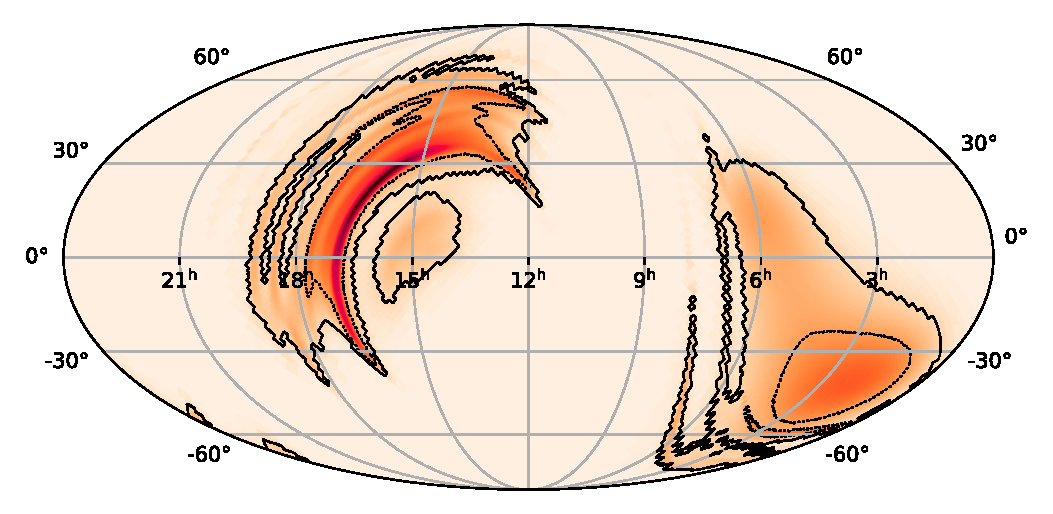
\includegraphics[width=0.8\linewidth]{images/tiling/gal_before.pdf}
        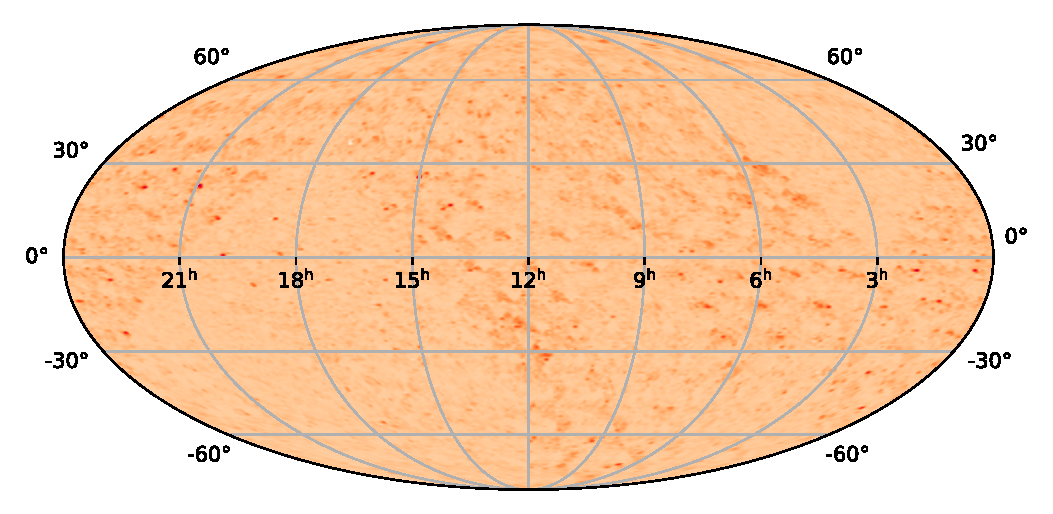
\includegraphics[width=0.8\linewidth]{images/tiling/gal.pdf}
        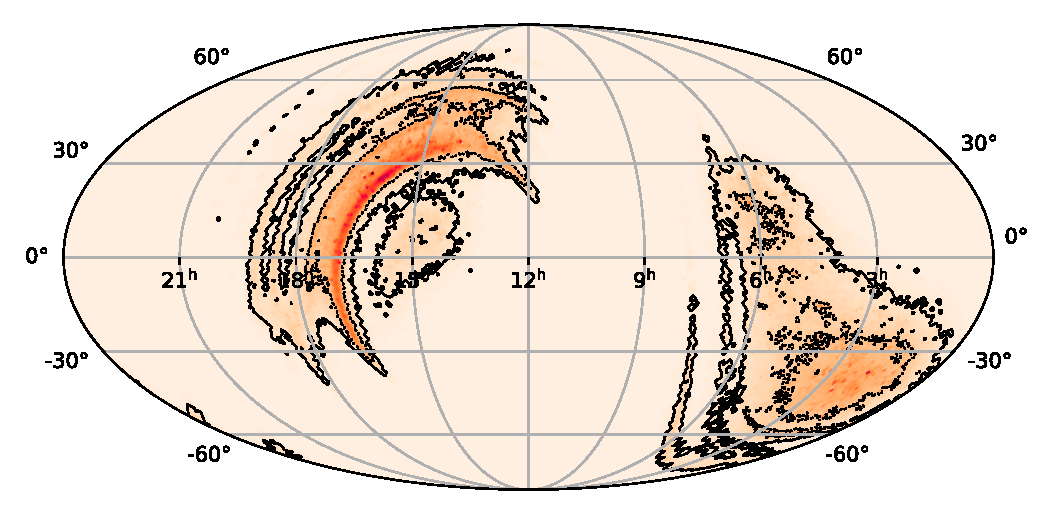
\includegraphics[width=0.8\linewidth]{images/tiling/gal_after.pdf}
    \end{center}
    \caption[Weighting a GW skymap using galaxy positions]{
        Weighting a GW skymap (for event S190425z) using galaxy positions. The top plot shows the BAYESTAR skymap distributed by the LVC, the central plot shows a skymap using GLADE galaxies within the estimated distance to the source ($155\pm\SI{45}{\mega\parsec}$), and the lower plot shows the result of multiplying the two together.
    }\label{fig:galaxy_skymap}
\end{figure}

\end{colsection}

% ~~~~~~~~~~~~~~~~~~~~

\subsection{Prioritising observations using dust extinction skymaps}
\label{sec:extinction_skymaps}
\begin{colsection}

In very crowded fields a single GOTO image can contain tens of thousands of sources, which makes it difficult for the GOTOphoto photometry pipeline (see \aref{sec:gotophoto}) to identify potential counterpart candidates. Observing in high-extinction areas such as through the galactic plane also makes it harder to observe extra-galactic sources, such as counterparts to gravitational-wave events. Therefore another possible reason to modify localisation skymaps is to de-prioritise observations of the galactic plane.

One method to do this is shown in \aref{fig:extinction_skymap} --- multiplying the gravitational-wave skymap by an inverted thermal dust emission skymap from the \textit{Planck} observatory \citep{Planck_dust}. The effect is intended to be subtle, not enough to completely wipe out the skymap probability in the high-extinction regions, but instead just reduce the weighting of those tiles so GOTO first prioritises other areas. Again, this is not currently implemented into the scheduling system, but it is presented as another example of using skymaps to optimise observation prioritises.

\begin{figure}[p]
    \begin{center}
        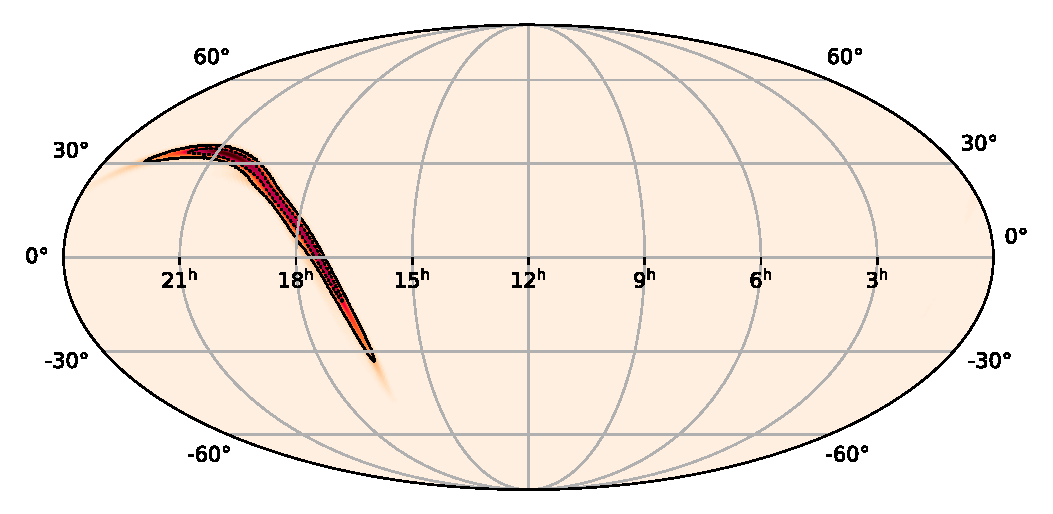
\includegraphics[width=0.8\linewidth]{images/tiling/ext_before.pdf}
        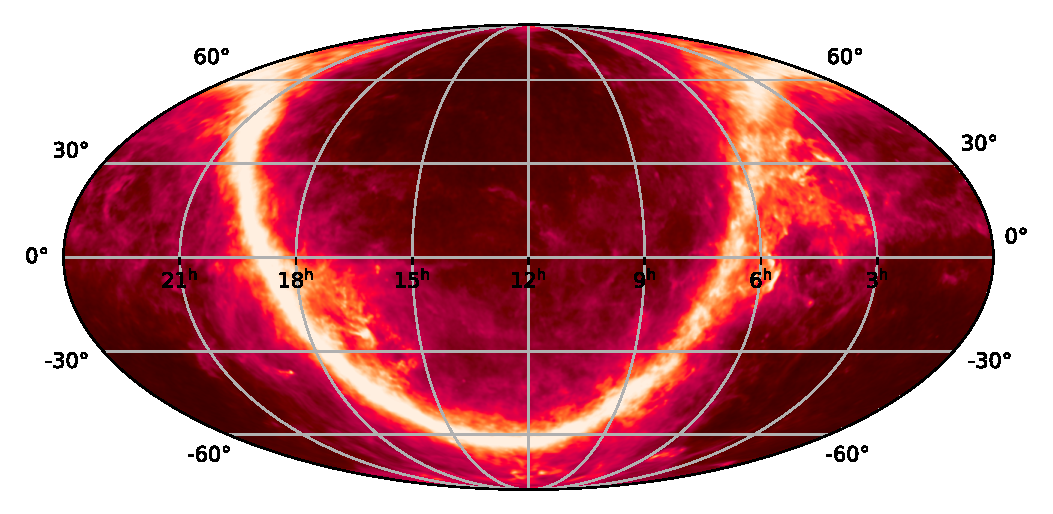
\includegraphics[width=0.8\linewidth]{images/tiling/ext.pdf}
        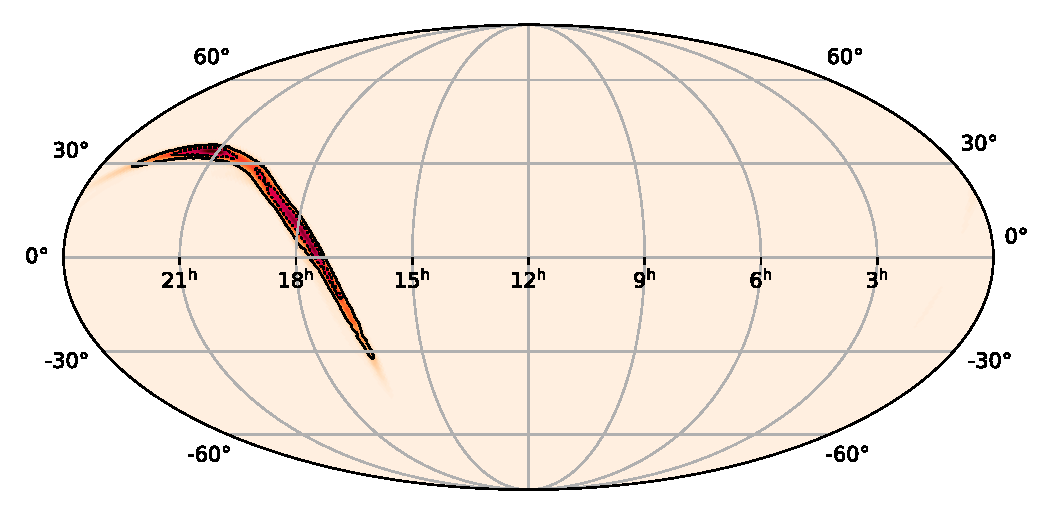
\includegraphics[width=0.8\linewidth]{images/tiling/ext_after.pdf}
    \end{center}
    \caption[Weighting a GW skymap using galactic extinction]{
        Weighting a GW skymap (for event S190521r) using galactic extinction. The top plot shows the BAYESTAR skymap distributed by the LVC, the central plot shows an inverted thermal dust emission skymap from \textit{Planck}, and the lower plot shows the result of multiplying the two together.
    }\label{fig:extinction_skymap}
\end{figure}

\end{colsection}

% ~~~~~~~~~~~~~~~~~~~~

\end{colsection}

% ########################################
